\documentclass[compress]{beamer}
\usepackage{ifthen,verbatim}

\newcommand{\isnote}{}
\xdefinecolor{lightyellow}{rgb}{1.,1.,0.25}
\xdefinecolor{darkblue}{rgb}{0.1,0.1,0.7}

%% Uncomment this to get annotations
%% \def\notes{\addtocounter{page}{-1}
%%            \renewcommand{\isnote}{*}
%% 	   \beamertemplateshadingbackground{lightyellow}{white}
%%            \begin{frame}
%%            \frametitle{Notes for the previous page (page \insertpagenumber)}
%%            \itemize}
%% \def\endnotes{\enditemize
%% 	      \end{frame}
%%               \beamertemplateshadingbackground{white}{white}
%%               \renewcommand{\isnote}{}}

%% Uncomment this to not get annotations
\def\notes{\comment}
\def\endnotes{\endcomment}

\setbeamertemplate{navigation symbols}{}
\setbeamertemplate{headline}{\mbox{ } \hfill
\begin{minipage}{5.5 cm}
\vspace{-0.75 cm} \small
\end{minipage} \hfill
\begin{minipage}{4.5 cm}
\vspace{-0.75 cm} \small
\begin{flushright}
\ifthenelse{\equal{\insertpagenumber}{1}}{}{Jim Pivarski \hspace{0.2 cm} \insertpagenumber\isnote/\pageref{numpages}}
\end{flushright}
\end{minipage}\mbox{\hspace{0.2 cm}}\includegraphics[height=1 cm]{../cmslogo} \hspace{0.1 cm} \includegraphics[height=1 cm]{../tamulogo} \hspace{0.01 cm} \vspace{-1.05 cm}}

\begin{document}
\begin{frame}
\vfill
\begin{center}
\textcolor{darkblue}{\Large Muon Alignment for Reprocessing}

\vfill
\begin{columns}
\column{0.3\linewidth}
\begin{center}
\large
\textcolor{darkblue}{Jim Pivarski}
\end{center}
\end{columns}

\begin{columns}
\column{0.3\linewidth}
\begin{center}
\scriptsize
{\it Texas A\&M University}
\end{center}
\end{columns}

\vfill
26 May, 2009

\end{center}
\end{frame}

%% \begin{notes}
%% \item This is the annotated version of my talk.
%% \item If you want the version that I am presenting, download the one
%% labeled ``slides'' on Indico (or just ignore these yellow pages).
%% \item The annotated version is provided for extra detail and a written
%% record of comments that I intend to make orally.
%% \item Yellow notes refer to the content on the {\it previous} page.
%% \item All other slides are identical for the two versions.
%% \end{notes}

\small

\begin{frame}
\frametitle{Consensus in muon alignment}
\begin{itemize}\setlength{\itemsep}{0.5 cm}
\item The muon alignment community has agreed upon an alignment update for the next reprocessing, to be proposed for sign-off tomorrow
\item It has three parts:
\begin{itemize}\setlength{\itemsep}{0.15 cm}
\item internal DT alignment
\item hardware $+$ photogrammetry CSC alignment
\item global chamber alignment for DT wheels $-$1, 0, $+$1
\end{itemize}
\item Global chamber alignment will need to be re-created with final tracker geometry and APEs
\begin{itemize}\setlength{\itemsep}{0.1 cm}\scriptsize
\item internal sign-off plots were all made with the nearly-final alignment
\item we do not expect large differences with the final tracker (geometry needs to be centered and APEs need to be updated)
\item we'll need to verify that the differences are small by HyperNews
\end{itemize}
\end{itemize}
%% \hspace{-0.83 cm} \textcolor{darkblue}{\Large Outline2}
\end{frame}

\begin{frame}
\frametitle{Internal DT alignment}

\begin{columns}
\column{0.4\linewidth}
\begin{itemize}
\item Physically-motivated correction (glue layer)
\item Track-based alignment method agrees with survey (540~$\mu$m in $\delta_z$)
\item Track-based constants proposed for sign-off
\end{itemize}

\column{0.6\linewidth}
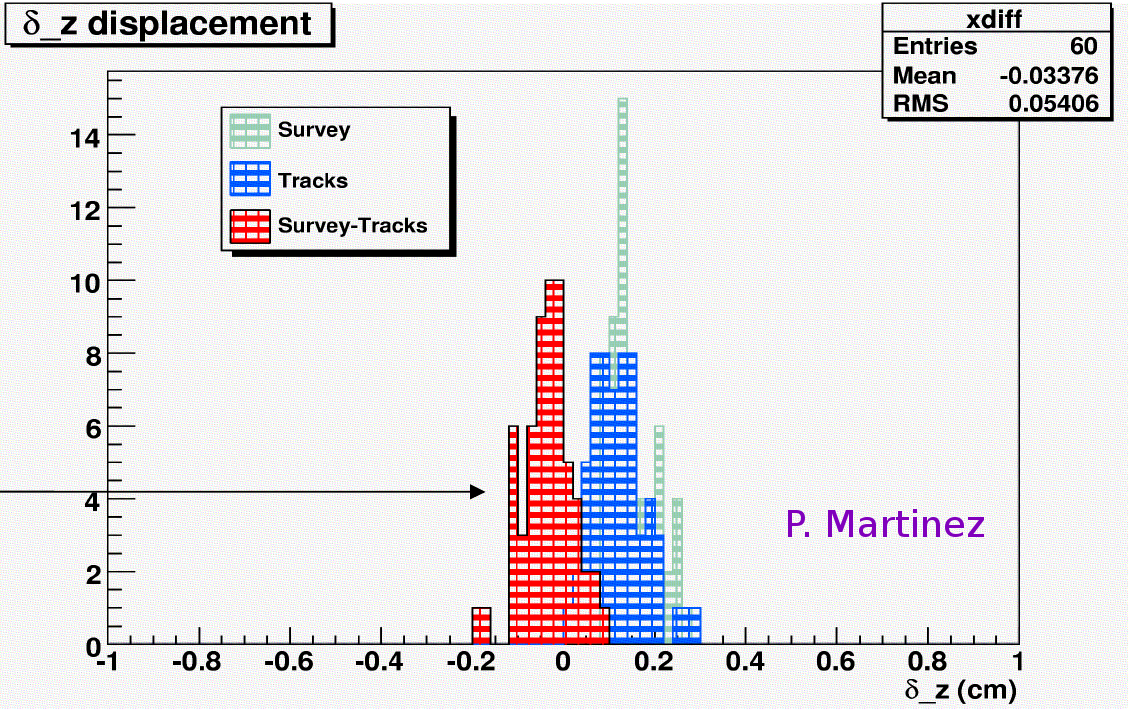
\includegraphics[width=\linewidth]{internal_alignment.png}
\end{columns}

\vfill
\hspace{-0.83 cm} \textcolor{darkblue}{\Large Hardware $+$ photogrammetry CSC alignment}

\begin{itemize}
\item Photogrammetry describes every chamber with $\vec{B}=0$~T
\item Hardware constants on top of PG describe disk-bending \mbox{in $\vec{B}=3.8$~T\hspace{-1 cm}}
\item All sign issues have been resolved; tracks have been re-fitted with the new constants
\end{itemize}

\hspace{-0.83 cm} \textcolor{darkblue}{Both of these were described in detail by Pablo on May 12; \mbox{they haven't changed\hspace{-1 cm}}}
\end{frame}

\begin{frame}
\frametitle{Global chamber alignment}

\begin{itemize}\setlength{\itemsep}{0.5 cm}
\item New since last alignment (CRAFT\_ALL\_V5--12, Jan 29):
\begin{itemize}\setlength{\itemsep}{0.1 cm}
\item combined fit to all 6 DOF, rather than independent $x$, $y$, $\phi_z$
\item well-defined region for alignment: wheels $-$1, 0, $+$1, all sectors except 1 and 7 (highest statistics)
\item high $p_T$ cut: 100--200~GeV, rather than 20--100~GeV
\end{itemize}
\item Studied in Monte Carlo (geometry-only, collisions, and cosmic rays)
\item Verification by different methods/groups:
\begin{itemize}\setlength{\itemsep}{0.1 cm}
\item tracker/globalMuon momentum ratio \hfill {\scriptsize (N.~Tran)}
\item cosmic ray splitting \hfill {\scriptsize (J.~Tucker and N.~Tran)}
\item segment extrapolation \hfill {\scriptsize (A.~Calderon)}
\end{itemize}
\end{itemize}
\end{frame}

\begin{frame}
\frametitle{Combined 6-DOF fit}

\begin{itemize}
\item Segment angle residuals ($\Delta \frac{dx}{dz}$ and $\Delta \frac{dy}{dz}$) give us more constraints
\end{itemize}

\vspace{-0.5 cm}
\[ \renewcommand{\arraystretch}{1.5}
\left(\begin{array}{c}
{\Delta x} \\
{\Delta y} \\
\textcolor{darkblue}{\Delta \frac{dx}{dz}} \\
\textcolor{darkblue}{\Delta \frac{dy}{dz}} \\
\end{array}\right)
=
\left(\begin{array}{c c c c c c}
-1 & \textcolor{white}{-}0 & \frac{dx}{dz} & y \frac{dx}{dz} & -x \frac{dx}{dz} & \textcolor{white}{-}y \\
\textcolor{white}{-}0 & -1 & \frac{dy}{dz} & y \frac{dy}{dz} & -x \frac{dy}{dz} & -x \\
\textcolor{white}{-}0 & \textcolor{white}{-}0 & 0 & \textcolor{darkblue}{\frac{dx}{dz} \frac{dy}{dz}} & \textcolor{darkblue}{-1 - \big(\frac{dx}{dz}\big)^2} & \textcolor{white}{-}\textcolor{darkblue}{\frac{dy}{dz}} \\
\textcolor{white}{-}0 & \textcolor{white}{-}0 & 0 & \textcolor{darkblue}{1 + \big(\frac{dy}{dz}\big)^2} & \textcolor{darkblue}{-\frac{dx}{dz}\frac{dy}{dz}} & \textcolor{darkblue}{-\frac{dx}{dz}}
\end{array}\right)
\renewcommand{\arraystretch}{1.05}
\left(\begin{array}{c}
\delta_x \\
\delta_y \\
\delta_z \\
\delta_{\phi_x} \\
\delta_{\phi_y} \\
\delta_{\phi_z}
\end{array}\right)
\]

\begin{columns}
\column{0.8\linewidth}
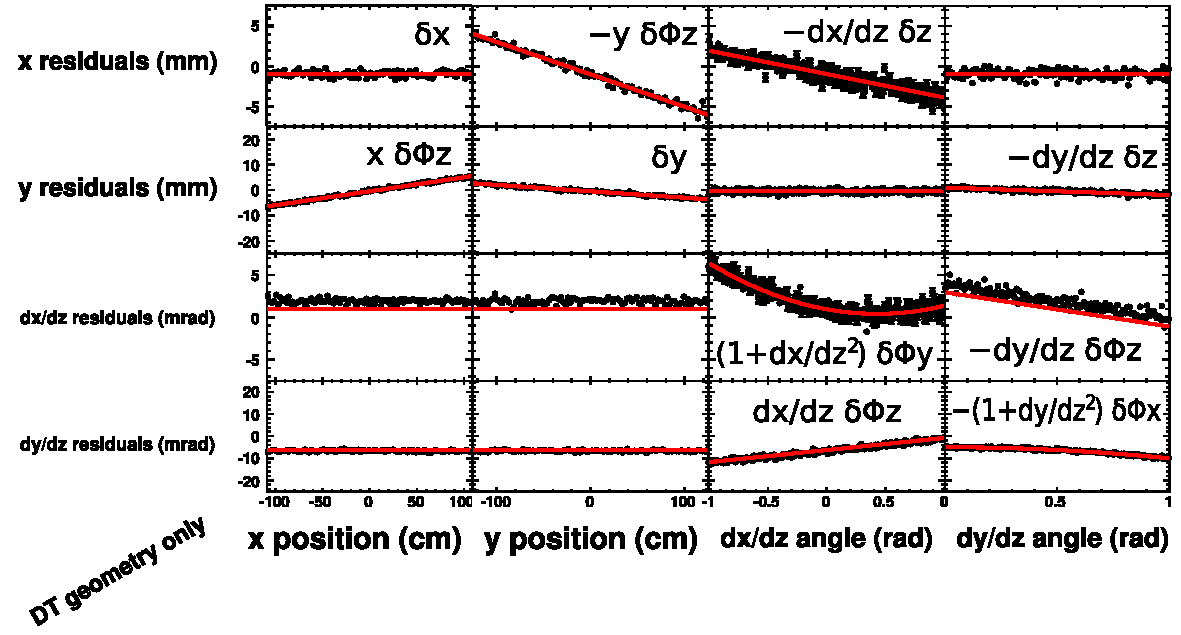
\includegraphics[width=\linewidth]{geometryonly_dt.pdf}
\column{0.3\linewidth}
\scriptsize
``Geometry-only MC'': concoction of CMSSW alignment tools and propagator to simulate alignment with no detector effects

\vspace{0.3 cm}
Validates our extension of the Karimaki derivative matrix (including signs)

\vspace{0.3 cm}
\end{columns}
\end{frame}

\begin{frame}
\frametitle{Example in full cosmics MC}
\begin{itemize}
\item Fit 4-D residuals distribution with all propagation effects included
\item 3-way convolution of alignment matrix, Gaussian errors, and Lorentzian scattering (8-D space, 16 parameters, check projections)
\end{itemize}

\mbox{\hspace{-0.85 cm}\begin{minipage}{1.1\linewidth}
\begin{tabular}{p{0.5\linewidth} p{0.5\linewidth}}
\mbox{ } \hfill \textcolor{darkblue}{\normalsize Before (misaligned)} \hfill \mbox{ } & \mbox{ } \hfill \textcolor{darkblue}{\normalsize After (aligned)} \hfill \mbox{ } \\
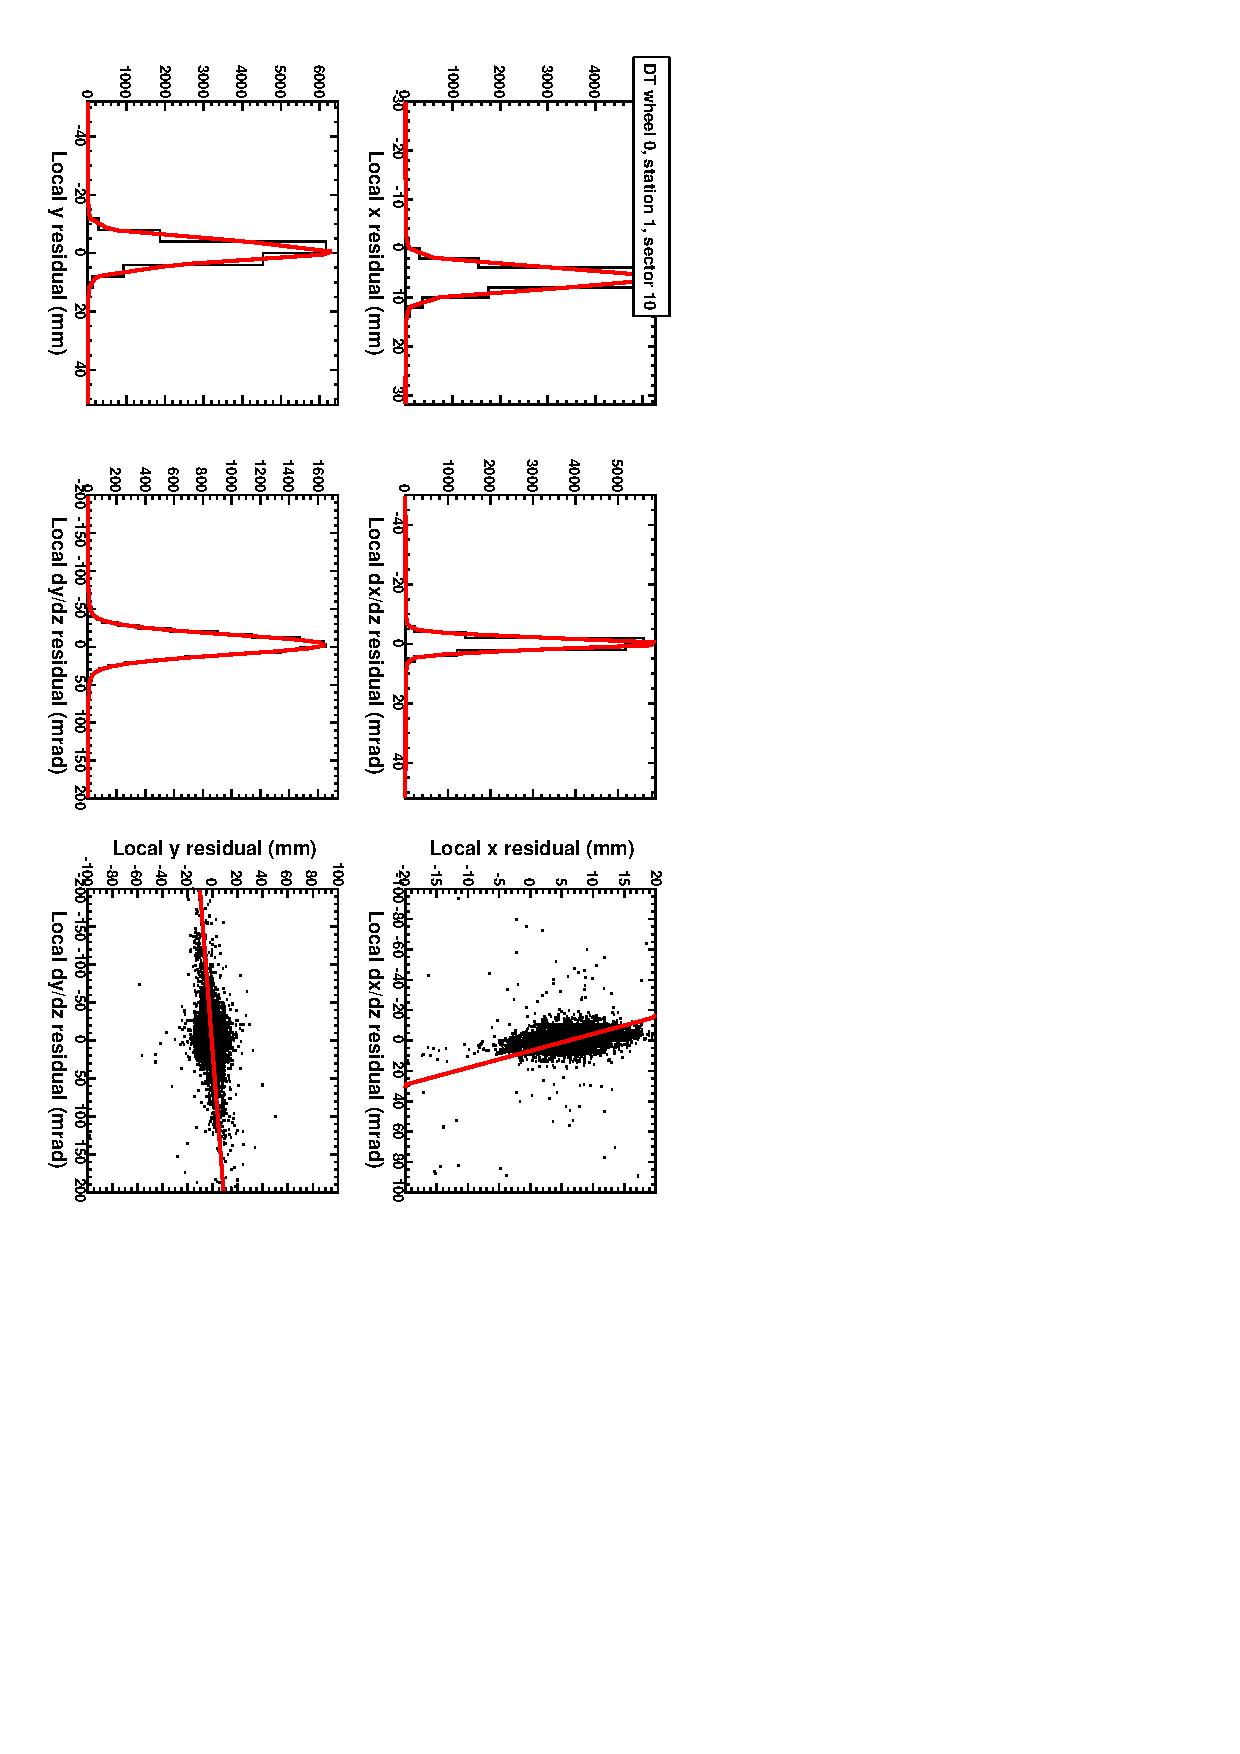
\includegraphics[height=\linewidth, angle=90]{exampleMC_wh0st1sec10_bellbefore.pdf} & 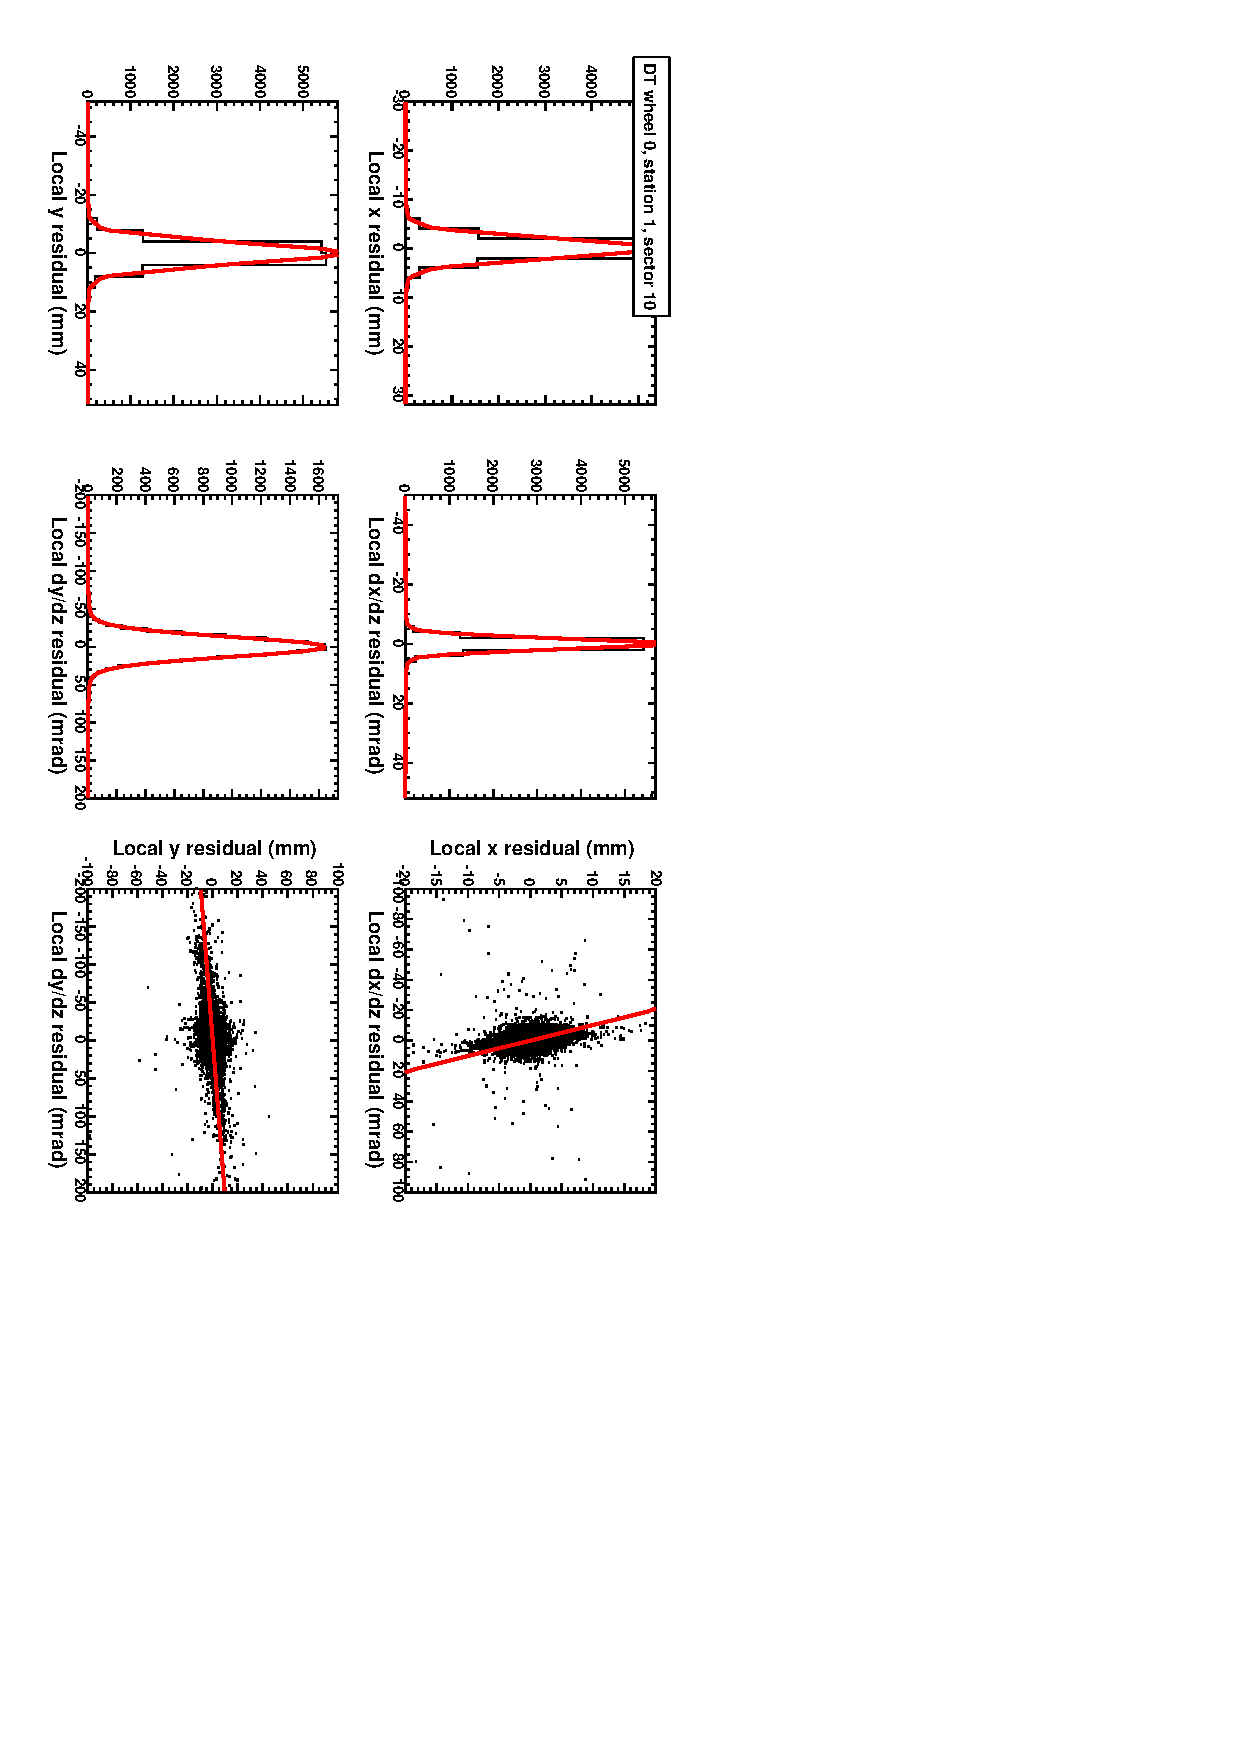
\includegraphics[height=\linewidth, angle=90]{exampleMC_wh0st1sec10_bellafter.pdf} \\
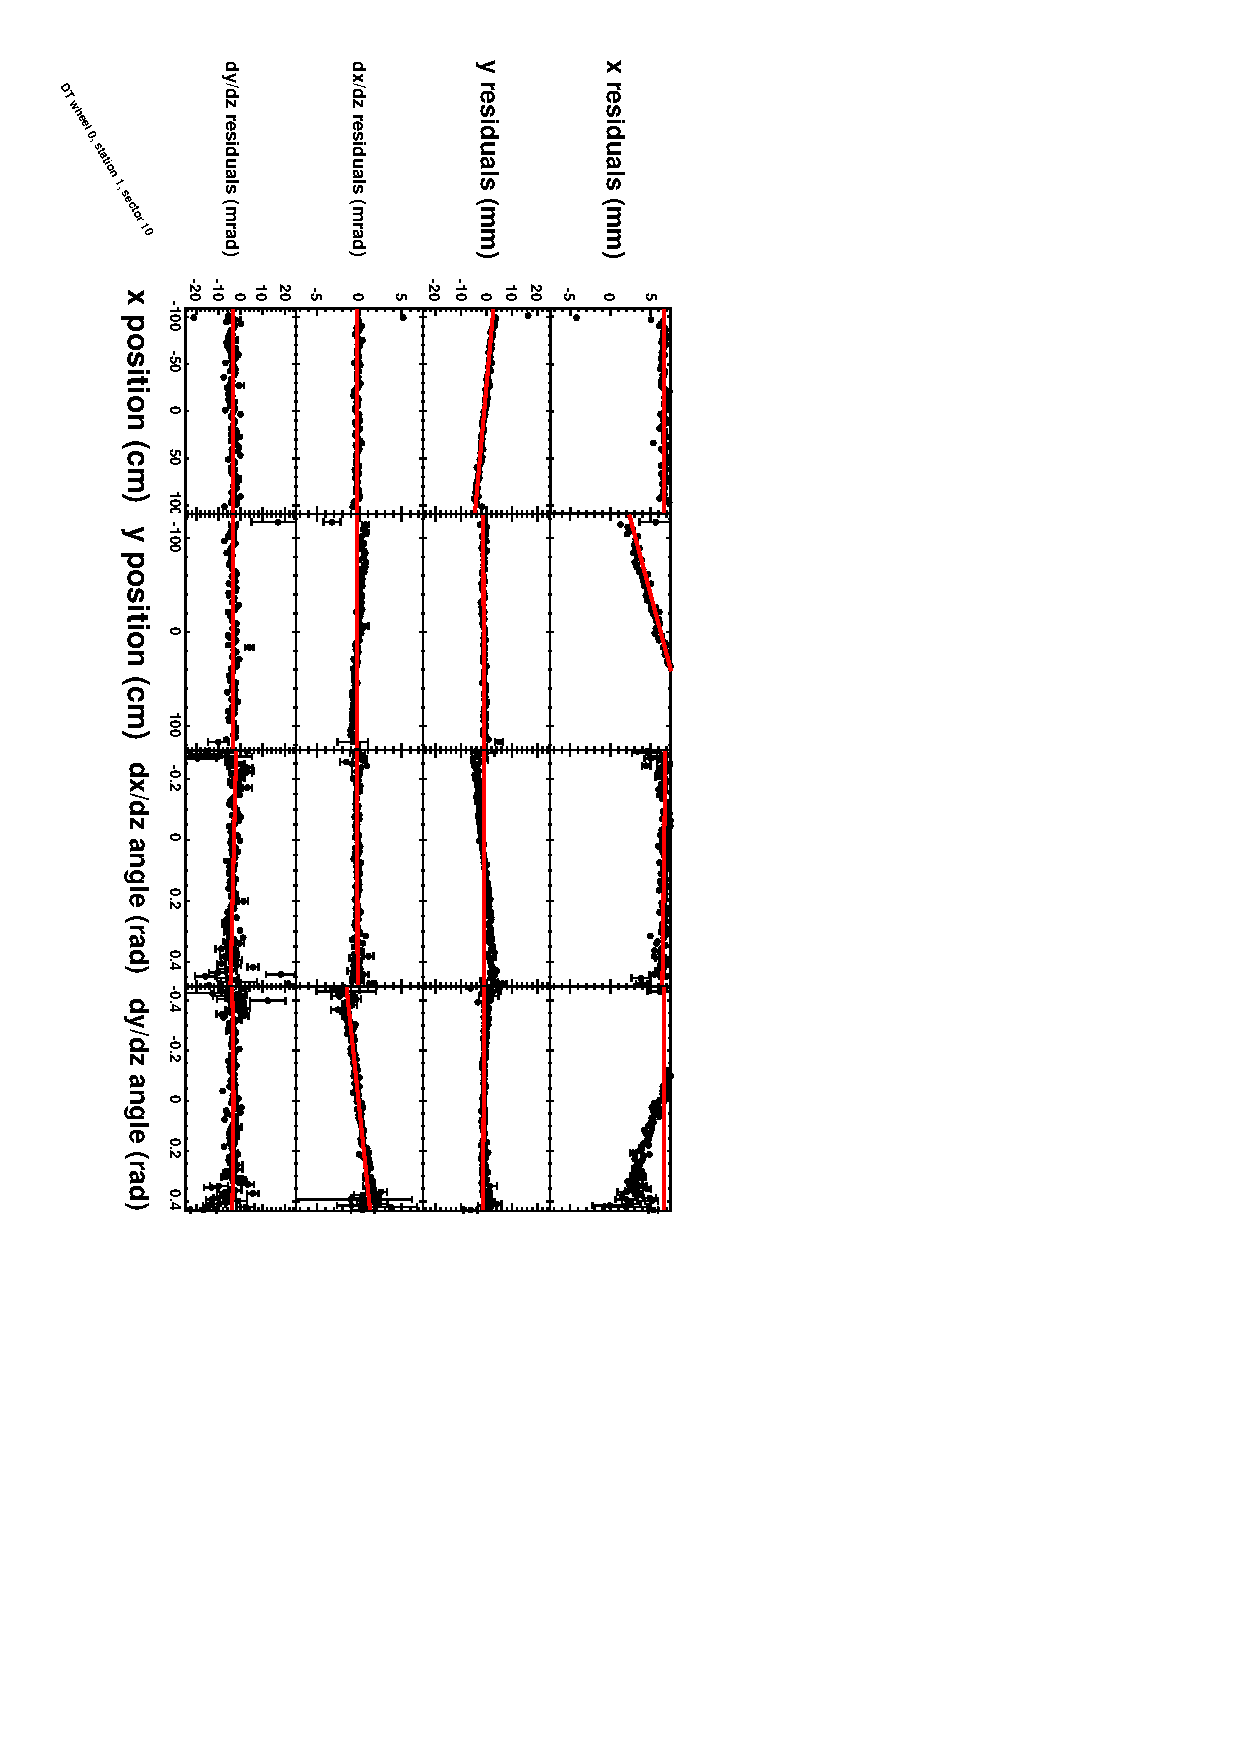
\includegraphics[height=\linewidth, angle=90]{exampleMC_wh0st1sec10_polybefore.pdf} & 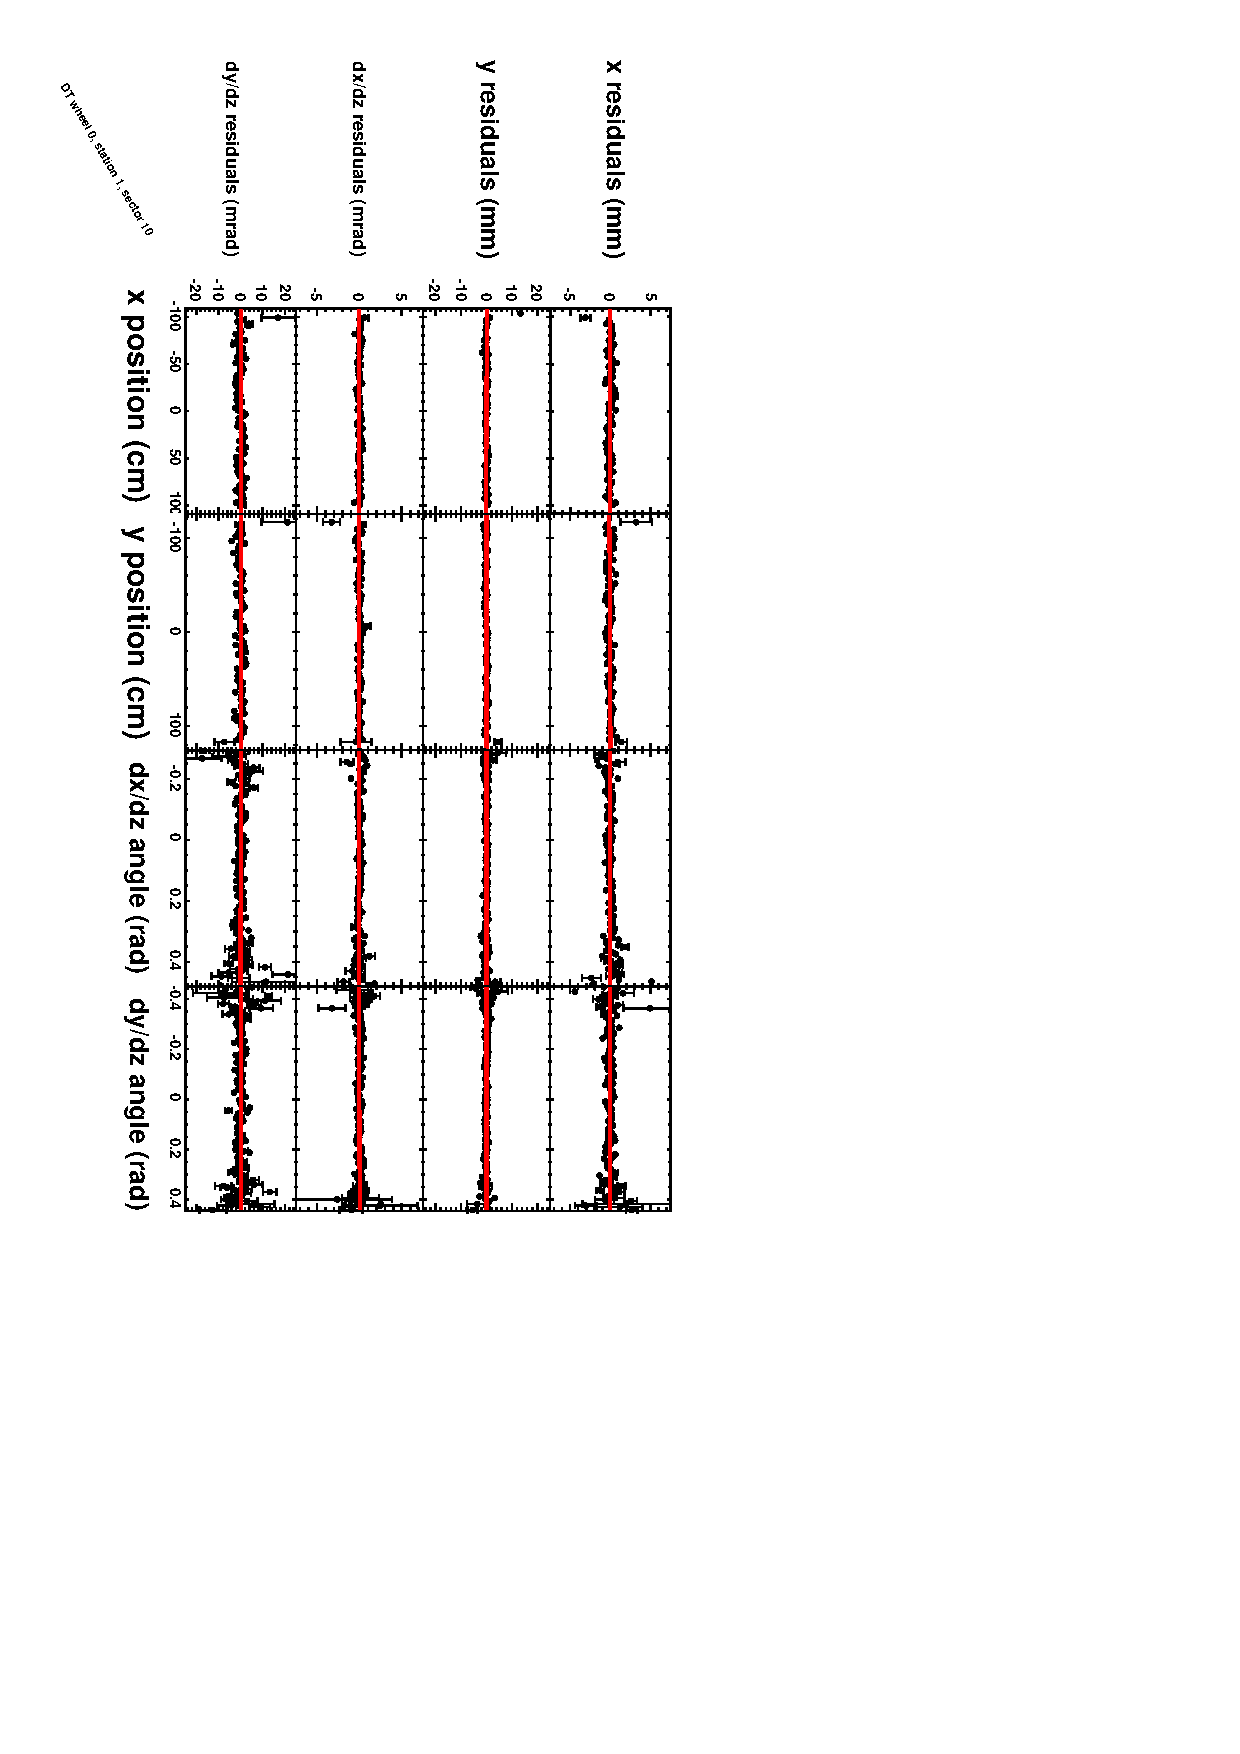
\includegraphics[height=\linewidth, angle=90]{exampleMC_wh0st1sec10_polyafter.pdf} \\
\end{tabular}\end{minipage}}
\end{frame}

\begin{frame}
\frametitle{Same example in real data}
\begin{itemize}
\item Wheel~0, station~1, sector~10 (largest statistics, bottom of CMS)
\end{itemize}

\vfill
\mbox{\hspace{-0.85 cm}\begin{minipage}{1.1\linewidth}
\begin{tabular}{p{0.5\linewidth} p{0.5\linewidth}}
\mbox{ } \hfill \textcolor{darkblue}{\normalsize Before (misaligned)} \hfill \mbox{ } & \mbox{ } \hfill \textcolor{darkblue}{\normalsize After (aligned)} \hfill \mbox{ } \\
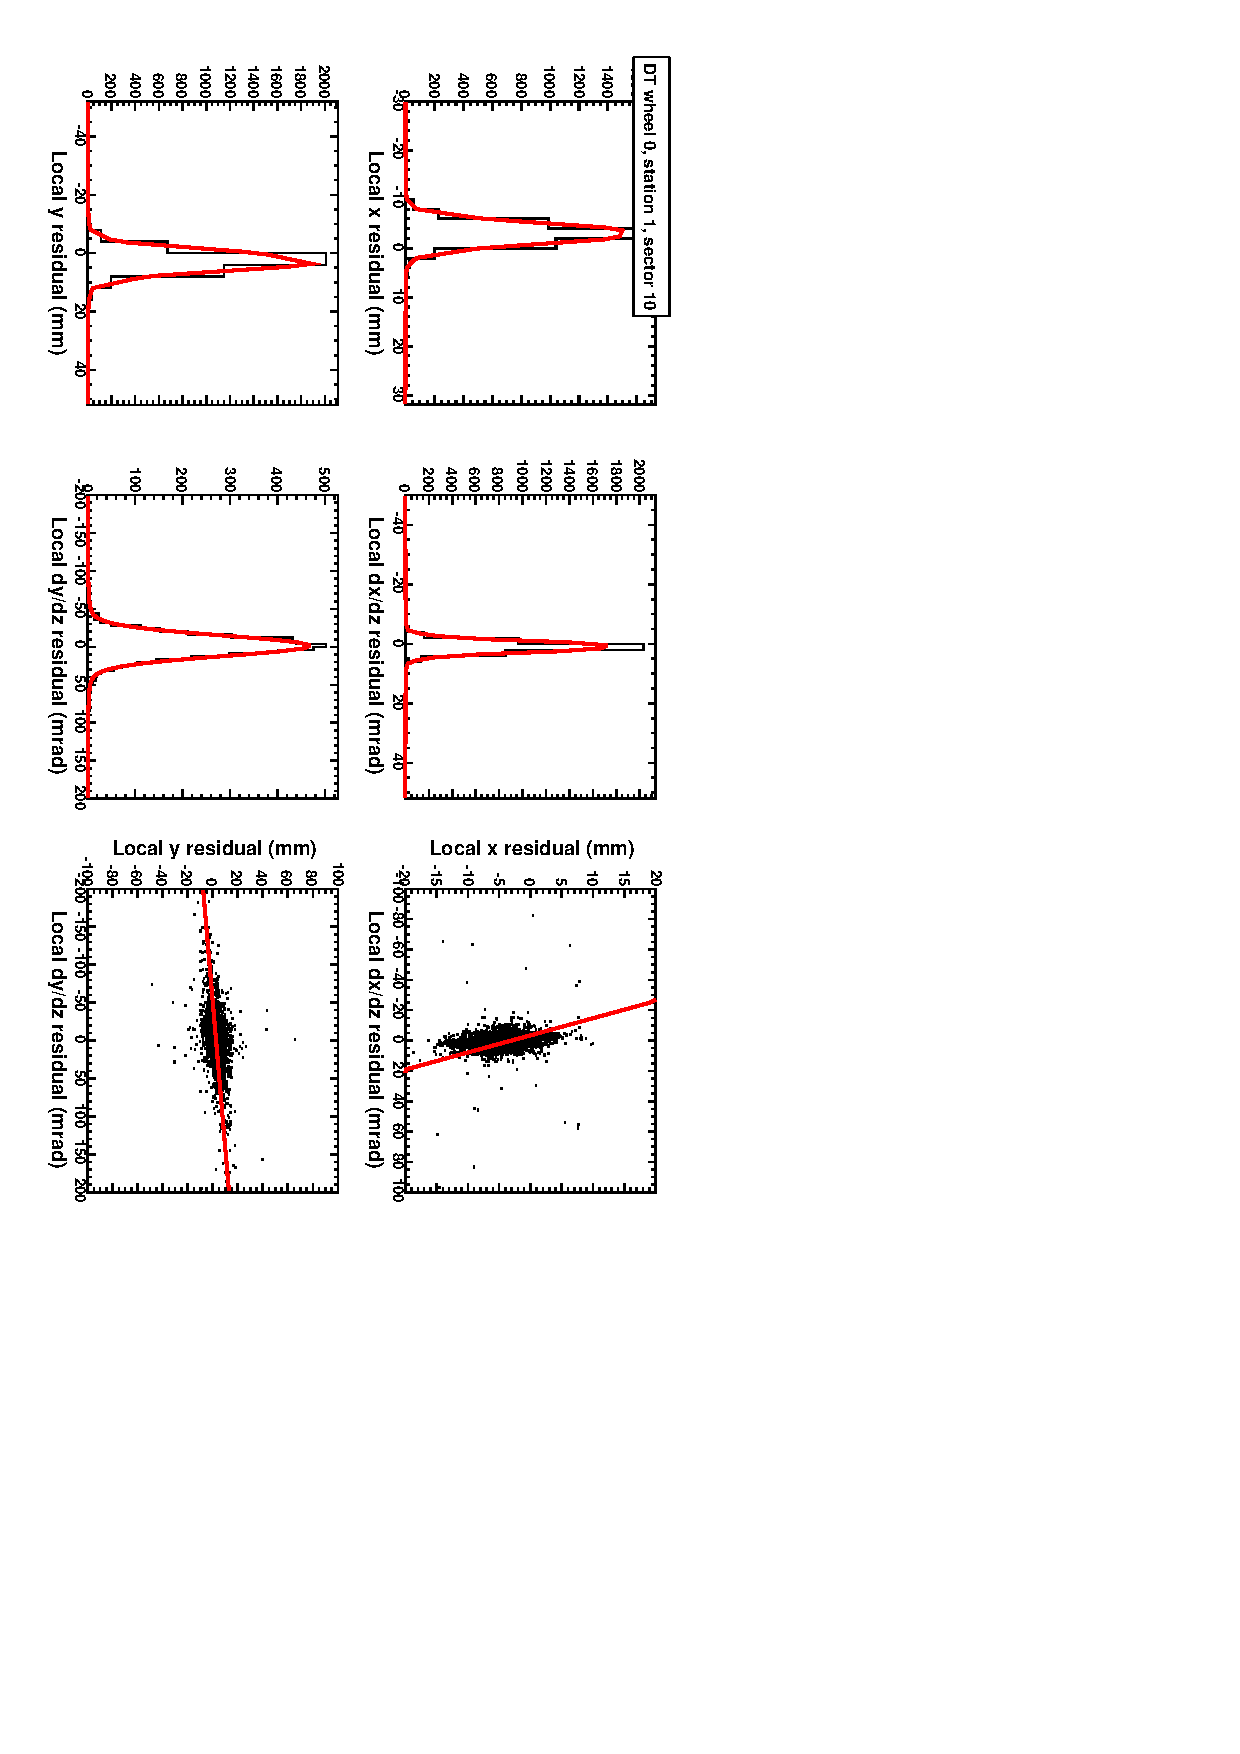
\includegraphics[height=\linewidth, angle=90]{exampleData_wh0st1sec10_bellbefore.pdf} & 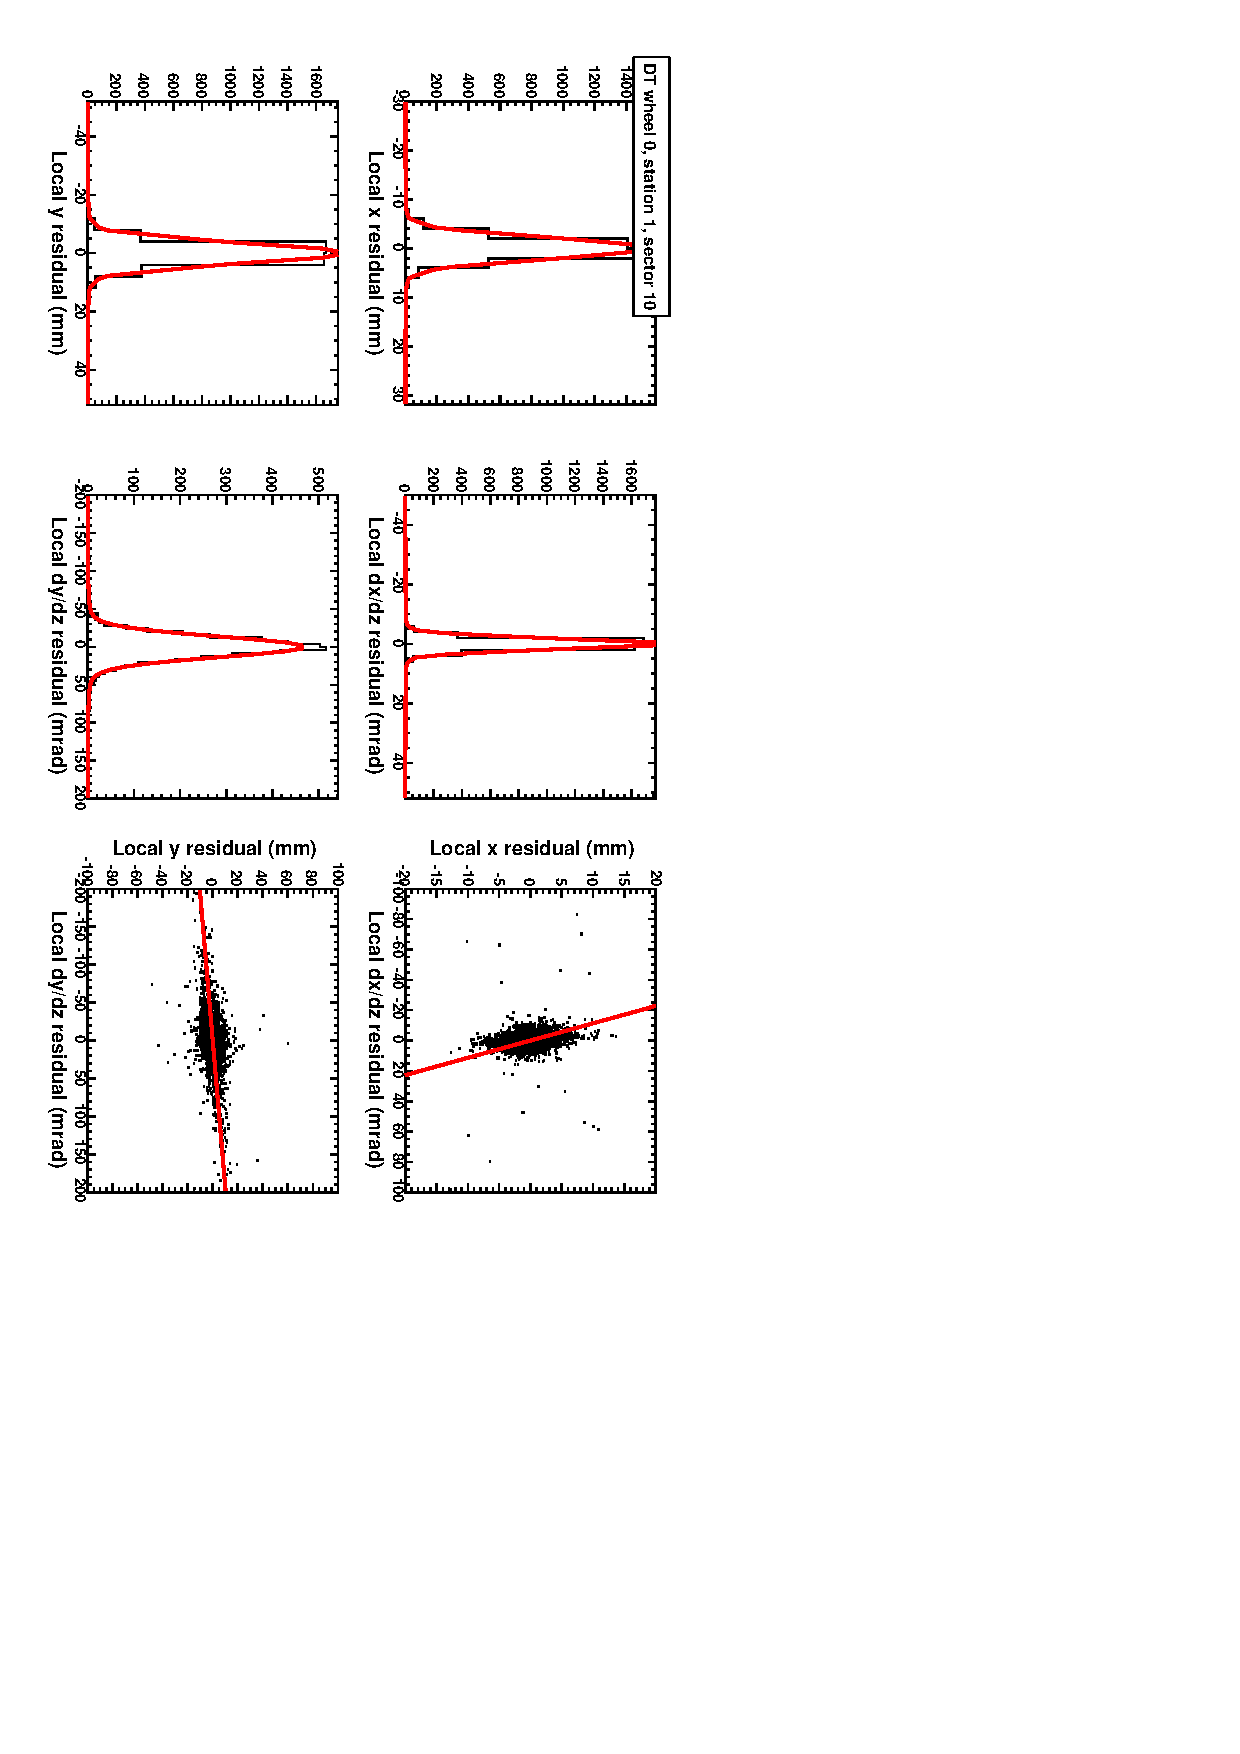
\includegraphics[height=\linewidth, angle=90]{exampleData_wh0st1sec10_bellafter.pdf} \\
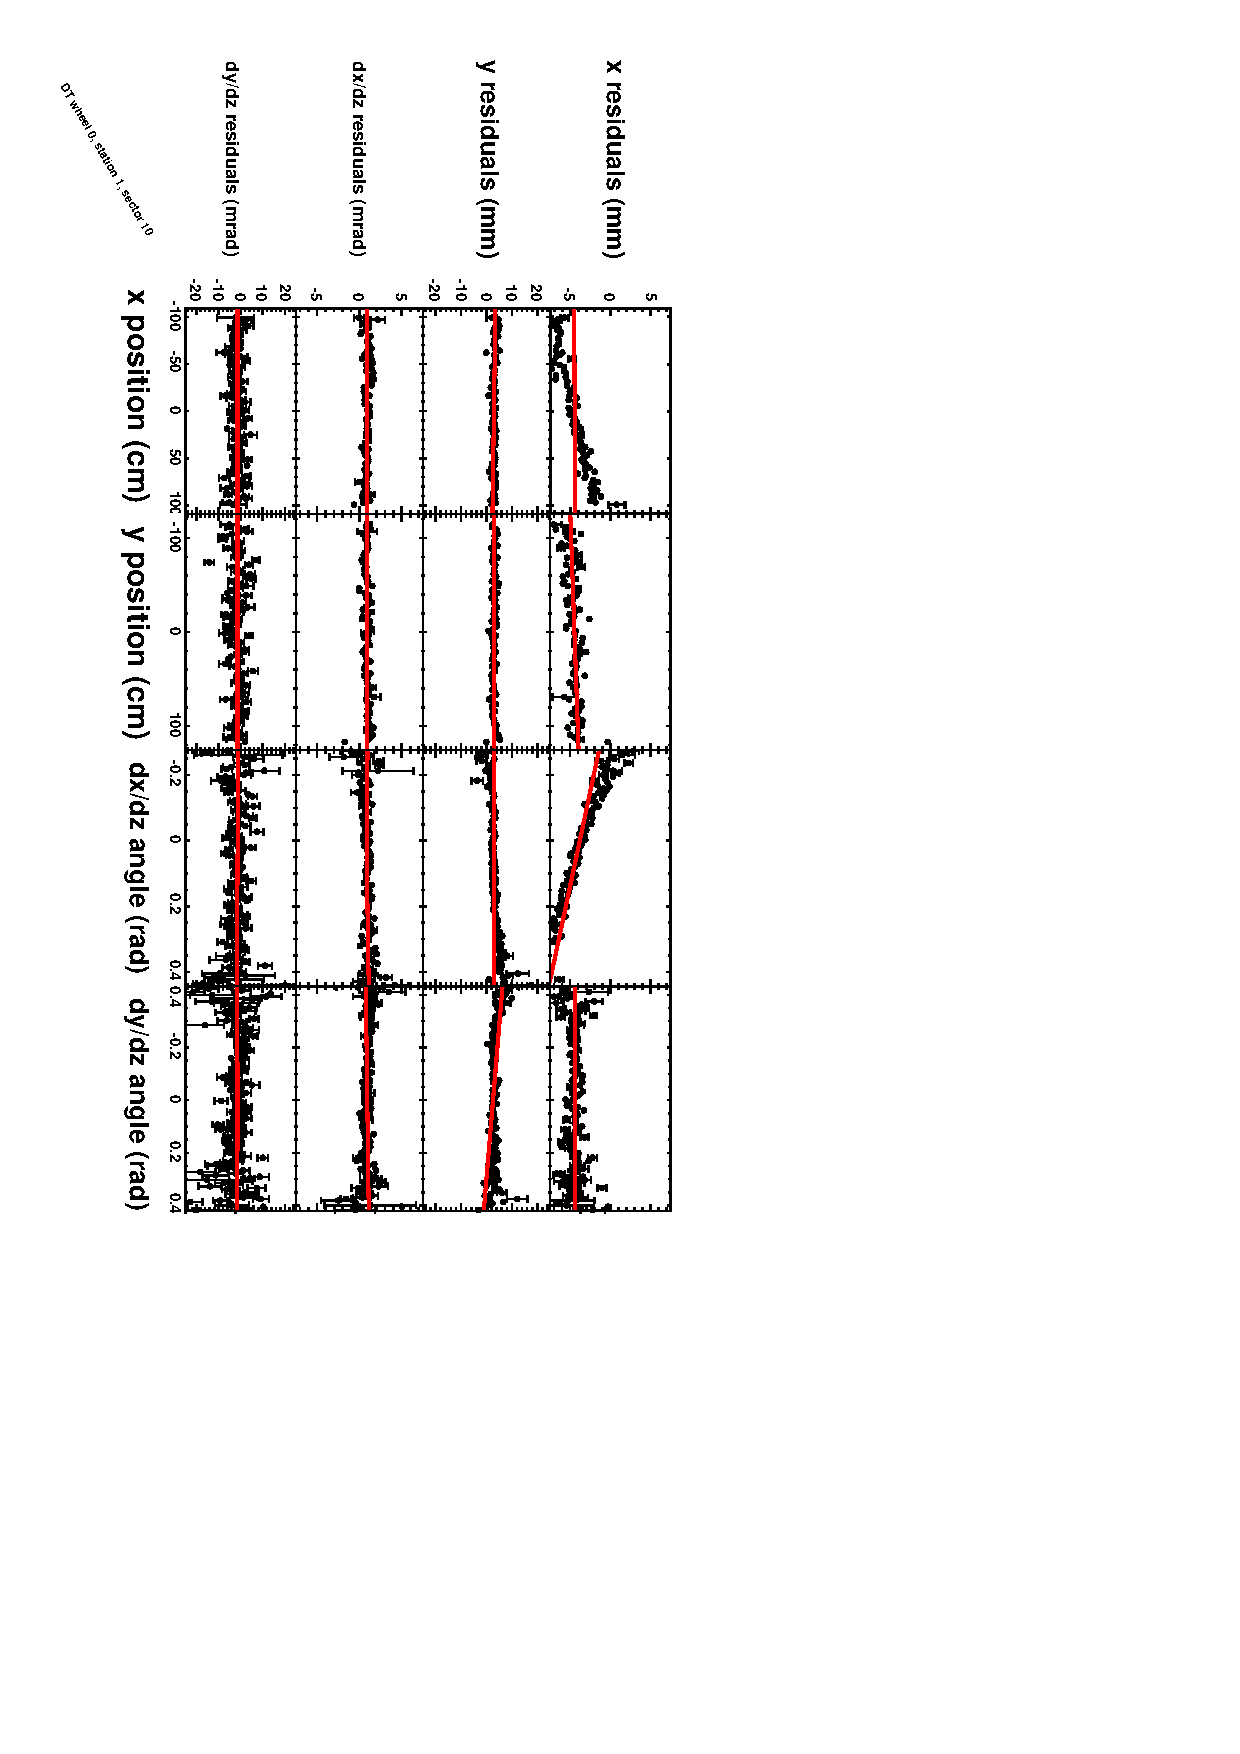
\includegraphics[height=\linewidth, angle=90]{exampleData_wh0st1sec10_polybefore.pdf} & 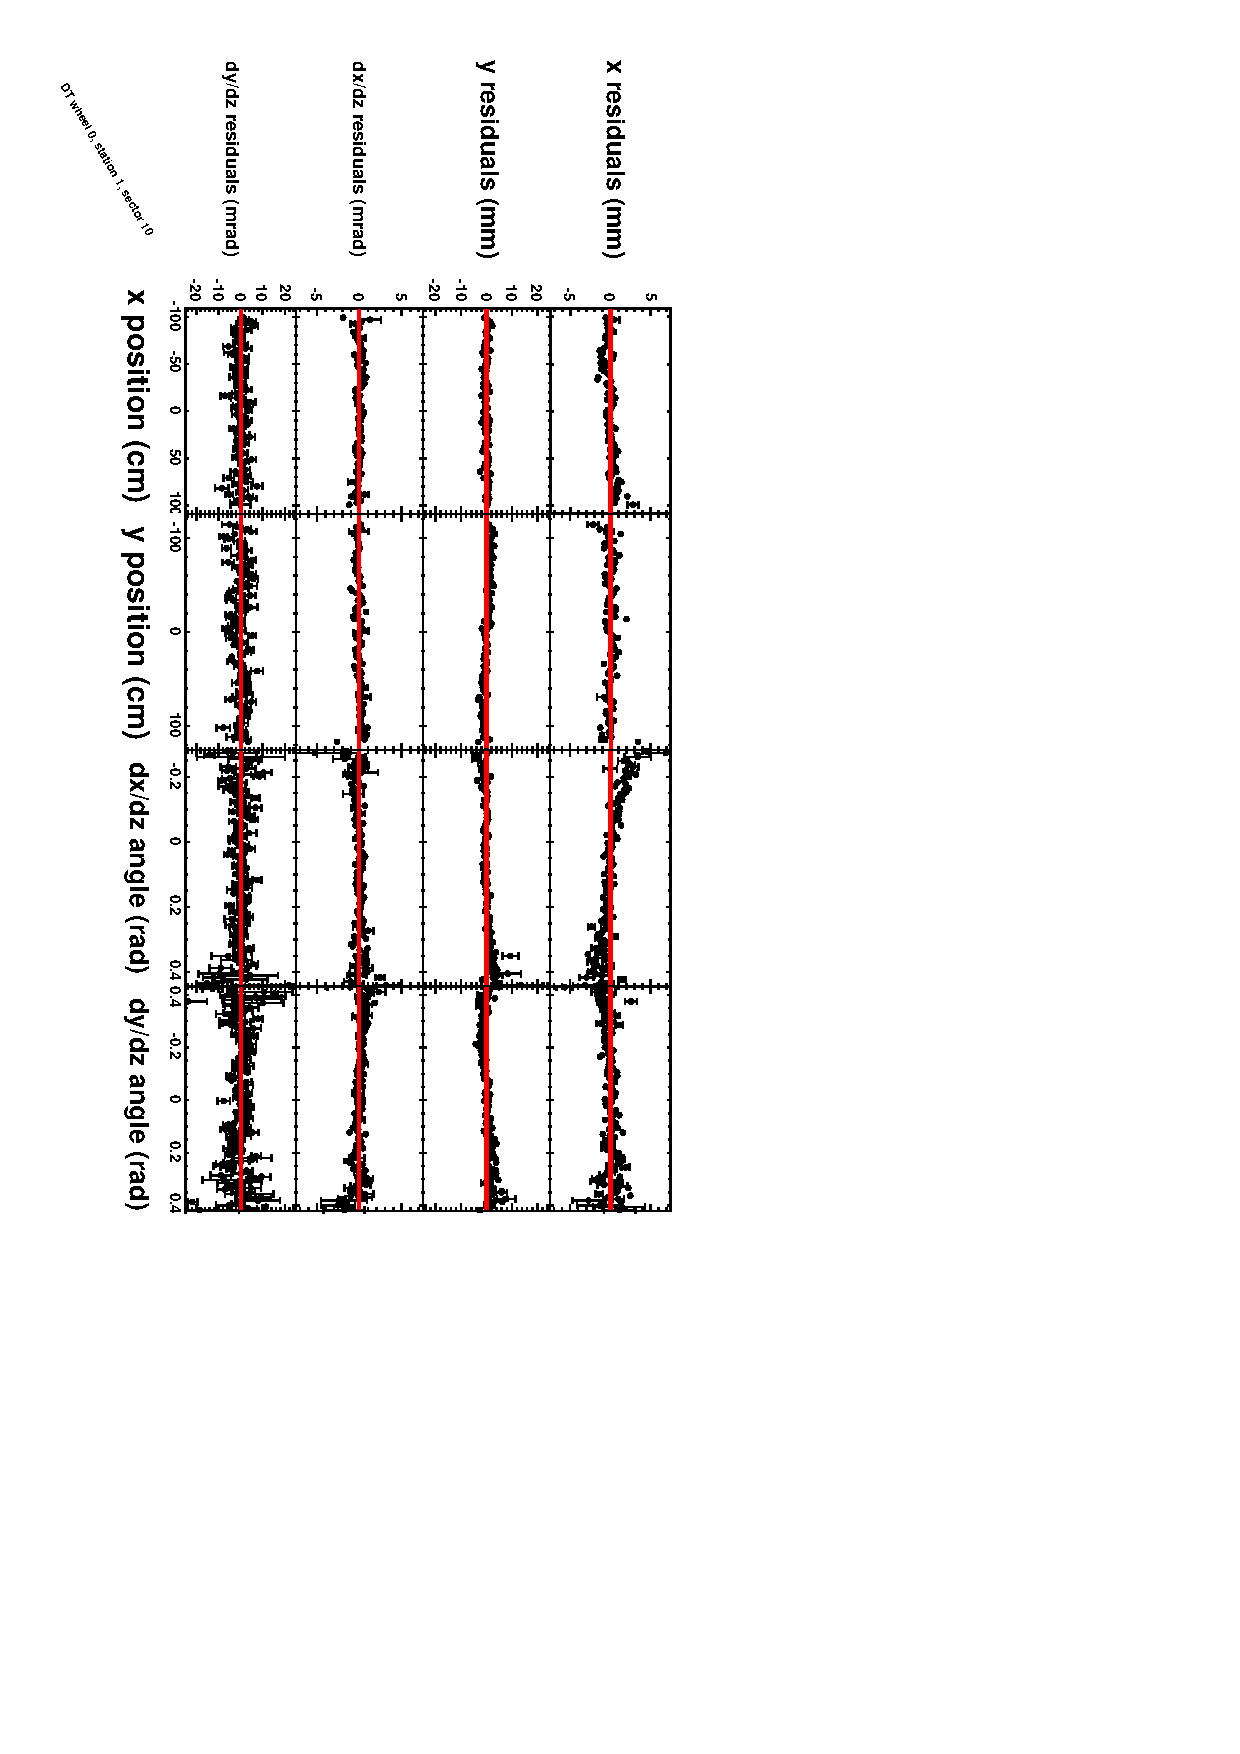
\includegraphics[height=\linewidth, angle=90]{exampleData_wh0st1sec10_polyafter.pdf} \\
\end{tabular}\end{minipage}}
\end{frame}

\begin{frame}
\frametitle{Accuracy in cosmics MC}
\begin{itemize}
\item All aspects of the MC alignment same as CRAFT except:
\begin{itemize}
\item ideal tracker, ideal $\vec{B}(\vec{x})$ map, ideal internal DT alignment
\item about 4 times the sample size
\end{itemize}
\item After 2 iterations, attain $r\phi$ accuracy of 200~$\mu$m
\end{itemize}

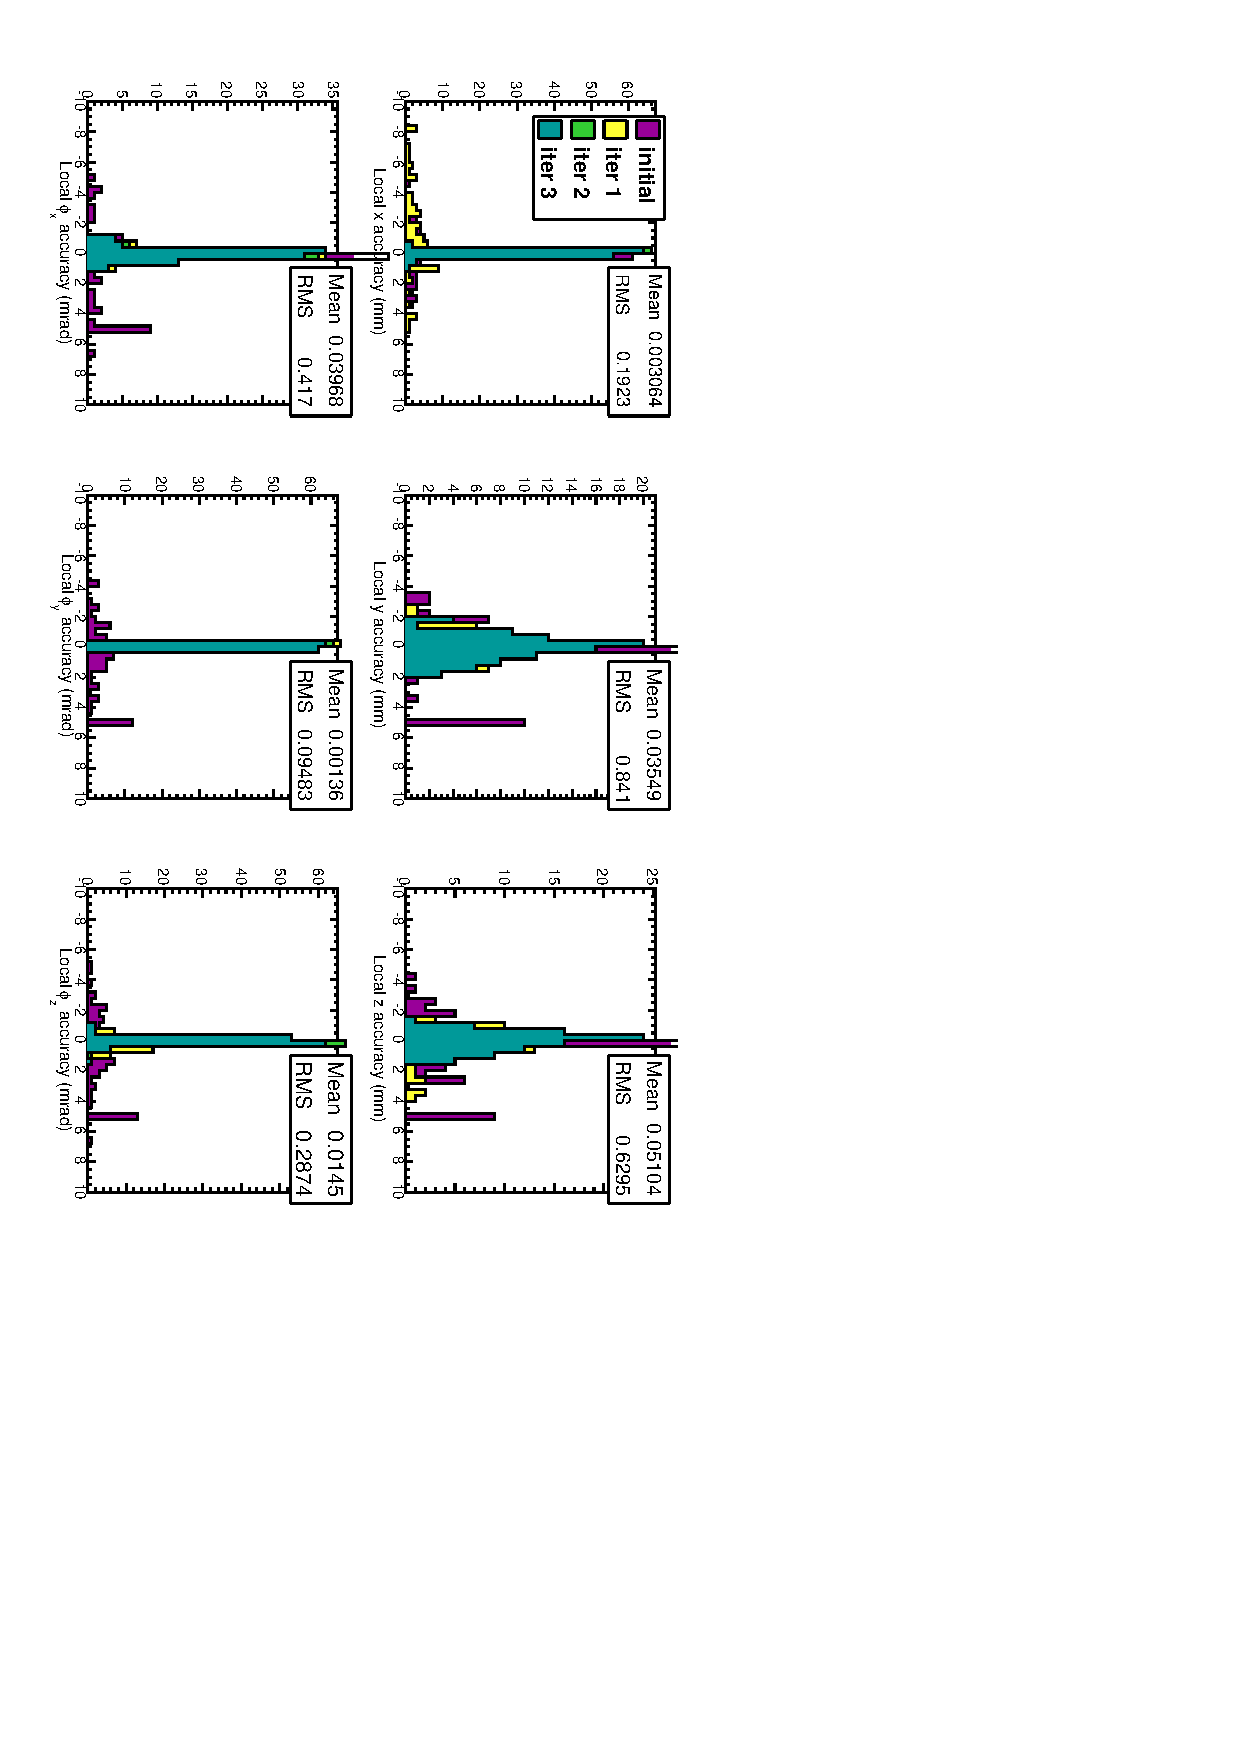
\includegraphics[height=\linewidth, angle=90]{hip_MC.pdf}
\end{frame}

\begin{frame}
\frametitle{Error analysis in MC}
\begin{itemize}
\item Statistical uncertainty from alignment fit is about 3--4 times smaller than differences between alignment and MC-truth
\item Define $\mbox{systematic error} = \sqrt{\mbox{(absolute error)}^2 - \mbox{(statistical)}^2}$
\begin{itemize}\setlength{\itemsep}{0.1 cm}
\item this ``systematic'' doesn't include unsimulated effects
\end{itemize}
\end{itemize}

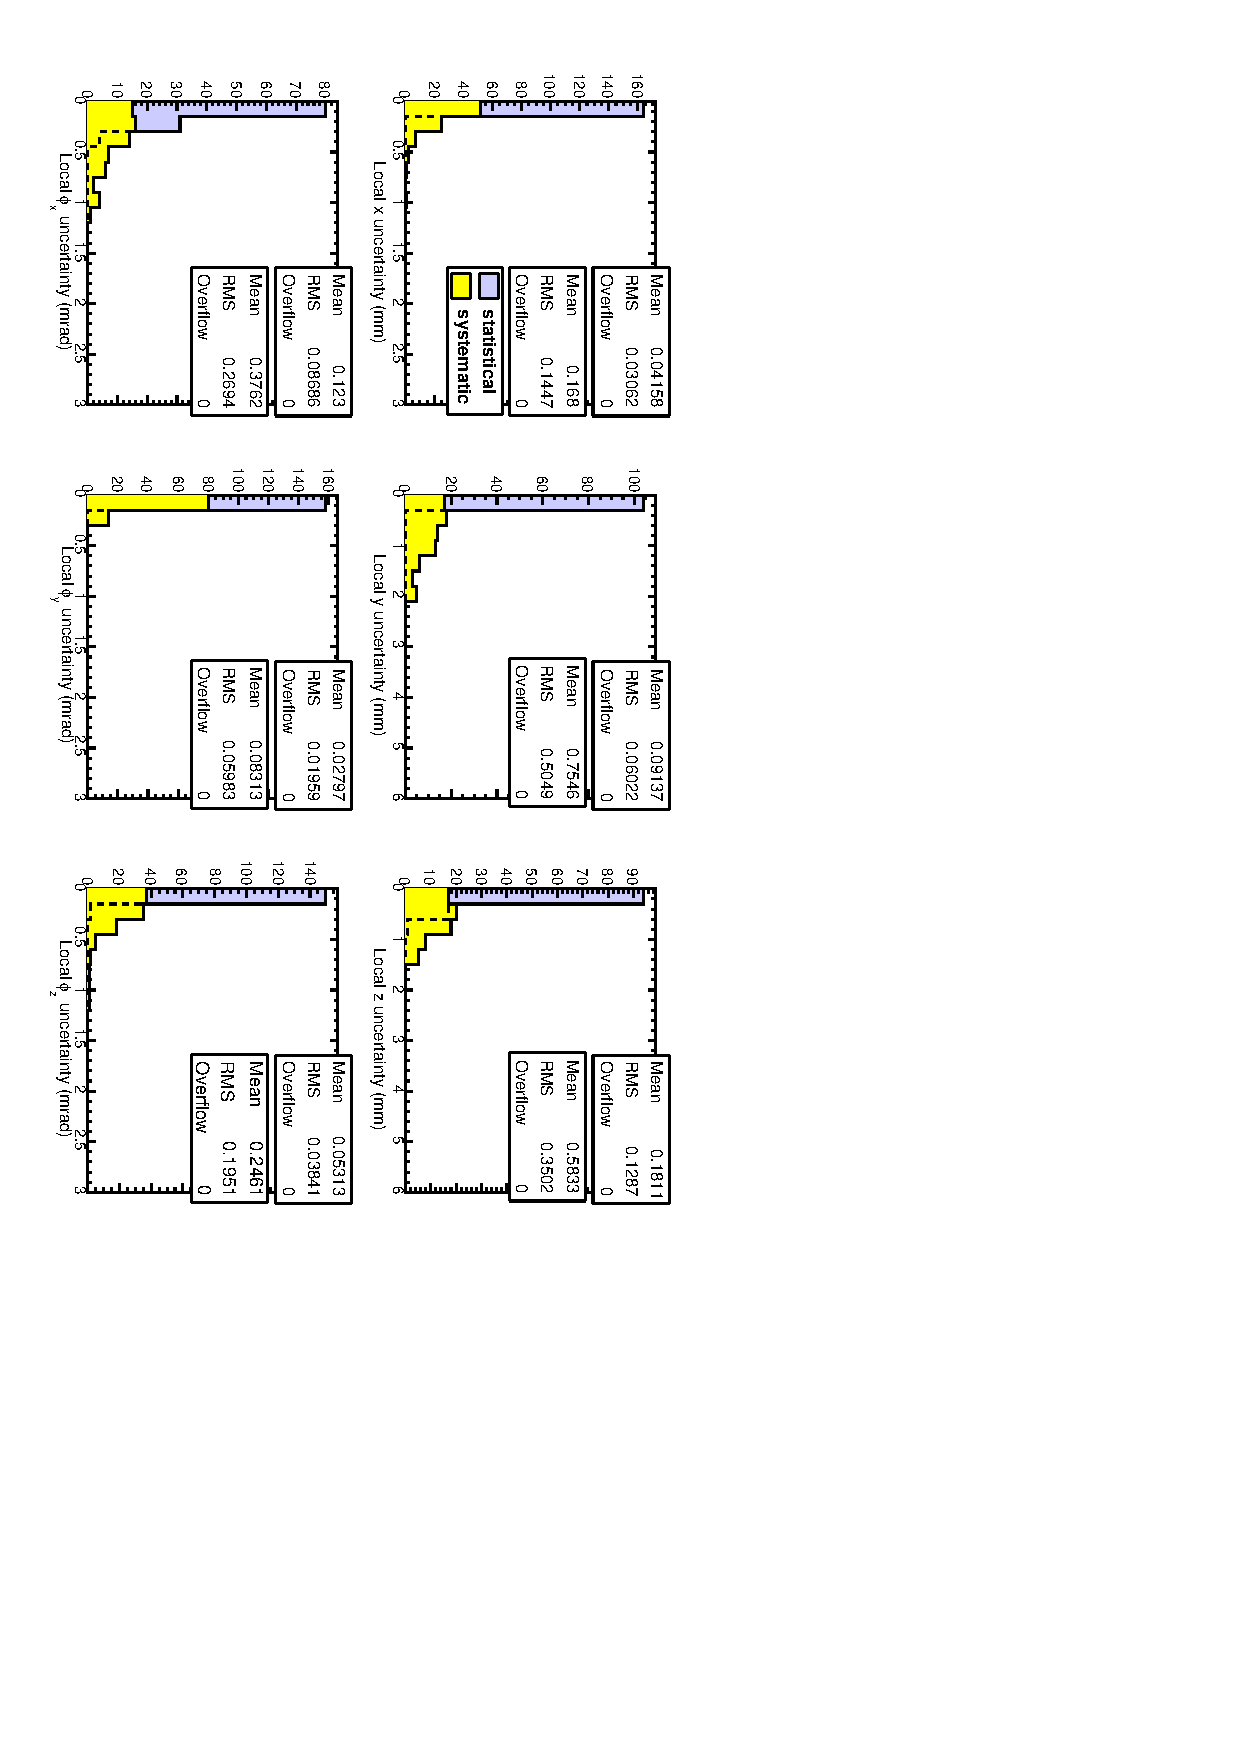
\includegraphics[height=\linewidth, angle=90]{hip_MCuncertainties.pdf}
\end{frame}

\begin{frame}
\frametitle{Dependence on $p_T$ cut}

\begin{columns}
\column{0.4\linewidth}
\vspace{0.1 cm}
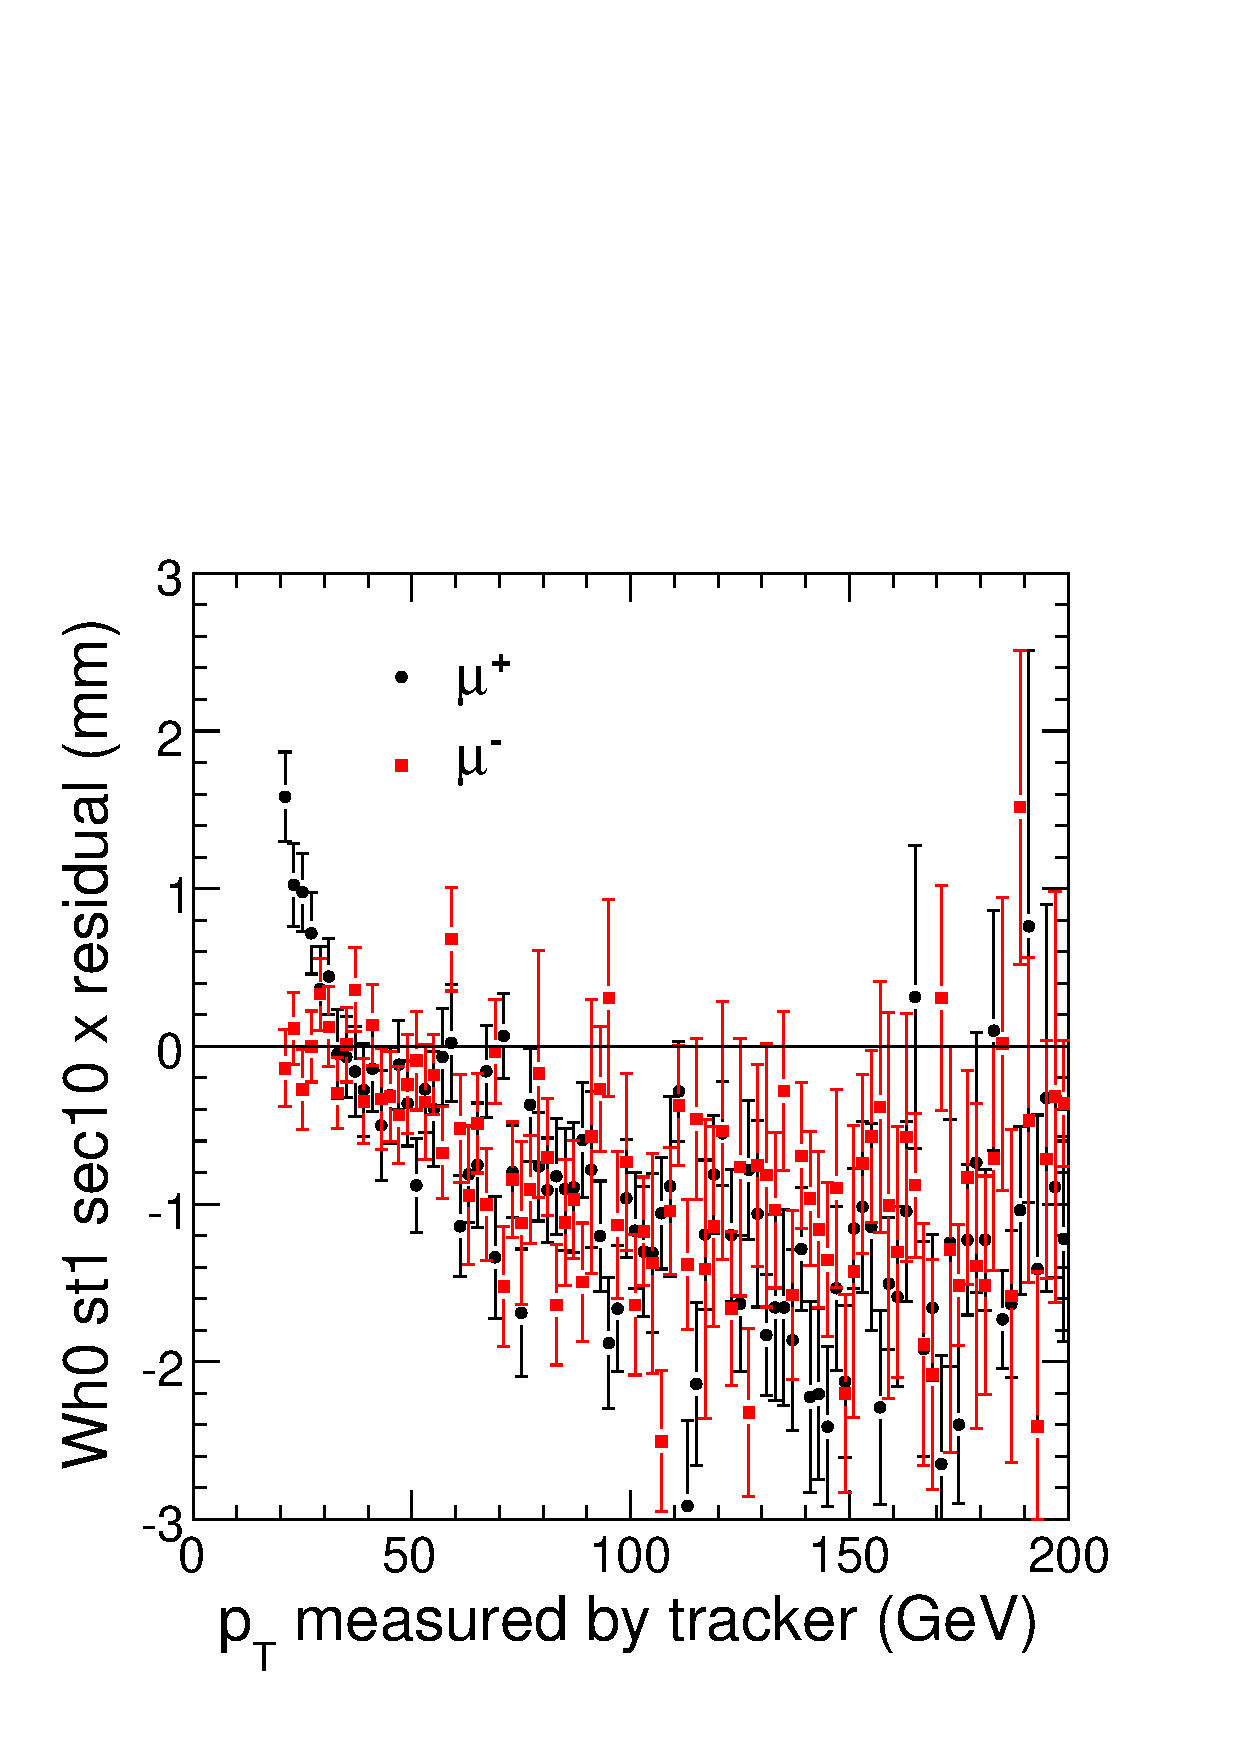
\includegraphics[width=\linewidth]{resid_vs_pt.pdf}

\begin{itemize}
\item Neither effect is present in Monte Carlo
\item Could be explained by tracker curl, but tracker studies already rule out the required magnitude (backup slides)
\end{itemize}

\column{0.6\linewidth}
\begin{itemize}
\item Expected and observed: splitting in residuals between $\mu^+$ and \textcolor{red}{$\mu^-$} at low momentum ($\vec{B}$ and $dE/dx$ effects)
\item Unexpected and observed: charge-independent variation in residuals at very high $p_T$
\item Dependence on $p_T$ and $\frac{dx}{dz}$ (sawtooth) are both unexplained and may be related
\end{itemize}

\vspace{-0.25 cm}
\hfill {\scriptsize Color scale: residuals (mm)}

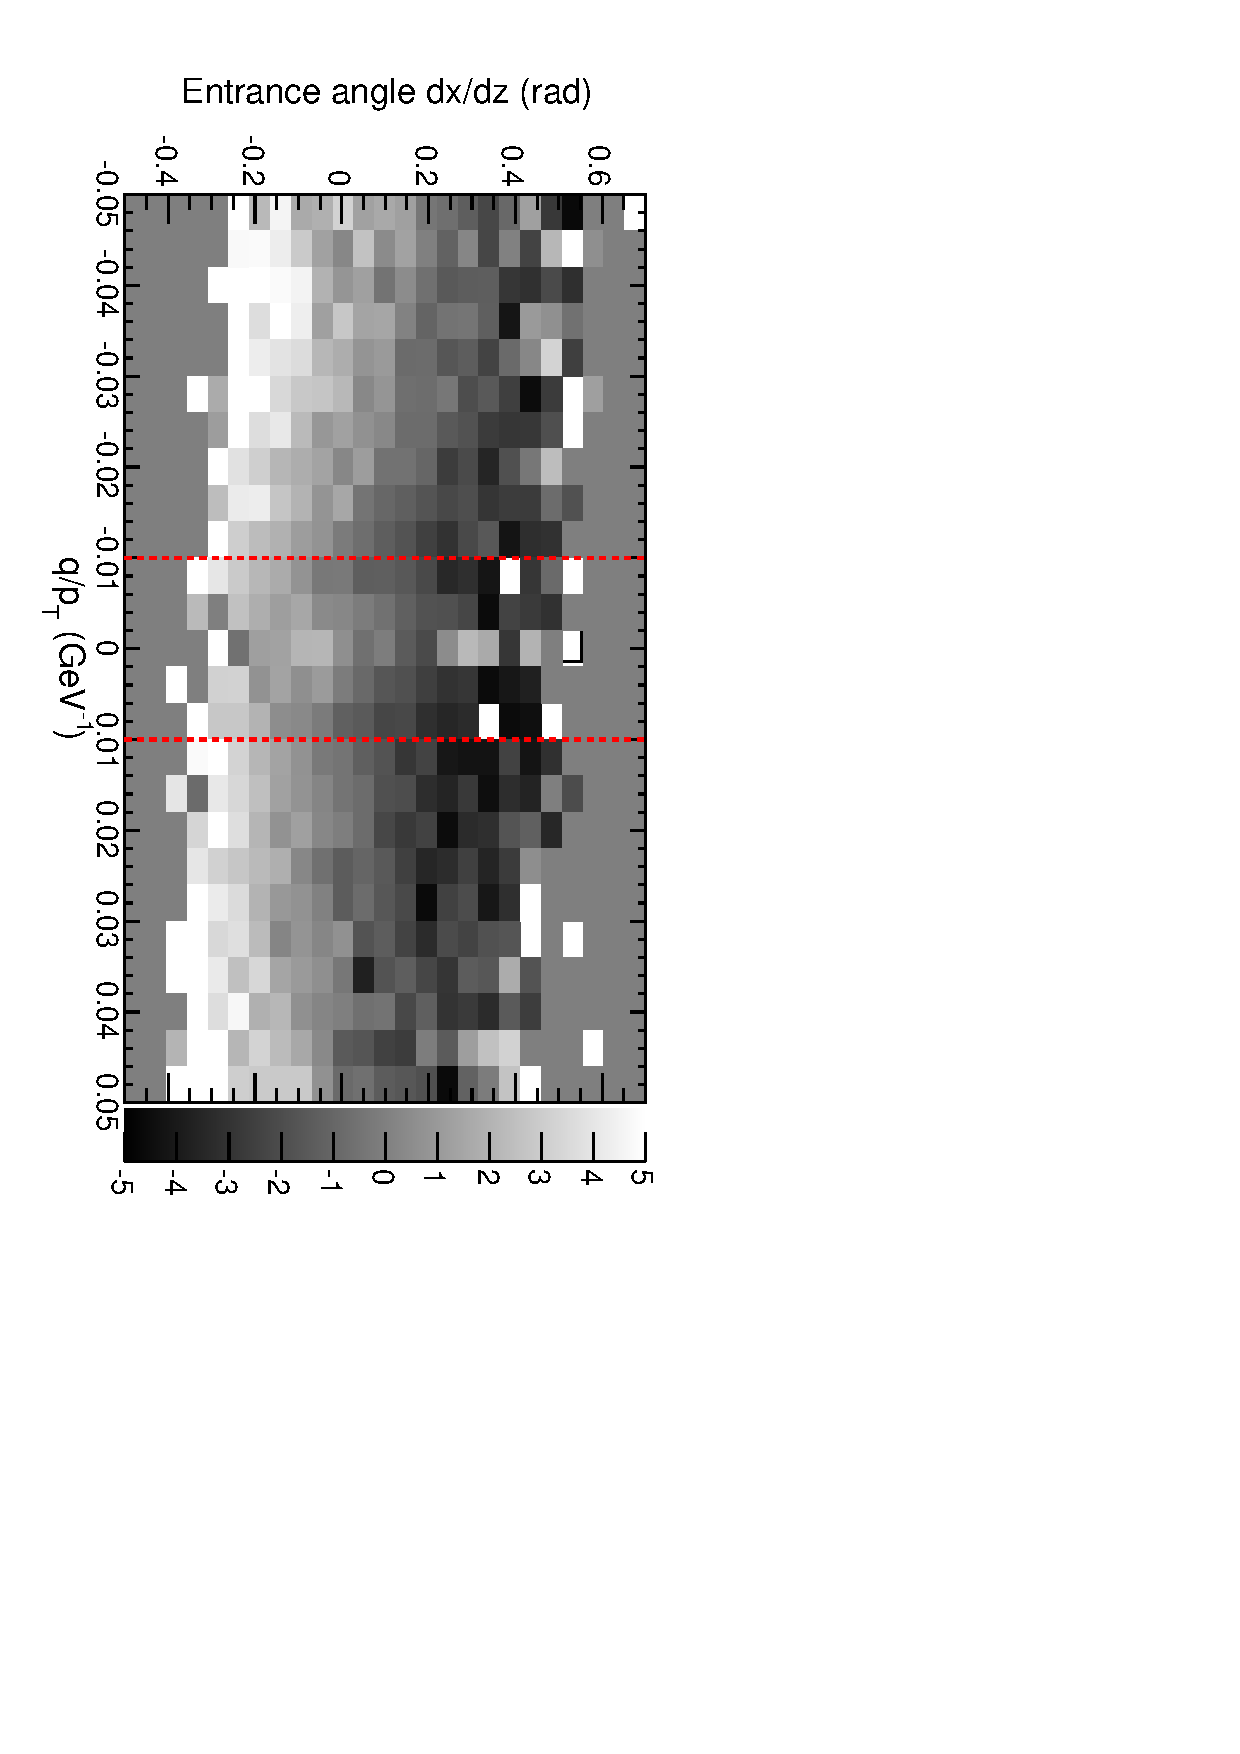
\includegraphics[height=\linewidth, angle=90]{sawtooth_qoverpt_complicated2.pdf}
\end{columns}
\end{frame}

\begin{frame}
\frametitle{Effect of $p_T$ cut on alignment}

\begin{itemize}
\item These plots show the difference between alignments produced with low $p_T$ (20--100~GeV) and high $p_T$ (100--200~GeV)
\begin{itemize}
\item global coordinates: $\Delta \phi$ (top row) is rotation around beamline, \\ $r\phi$ (bottom row) is the same orientation for all chambers
\end{itemize}
\item 0.35 mrad rotation, 0.04 mrad/m twist, and 3.2 mm spread
\end{itemize}

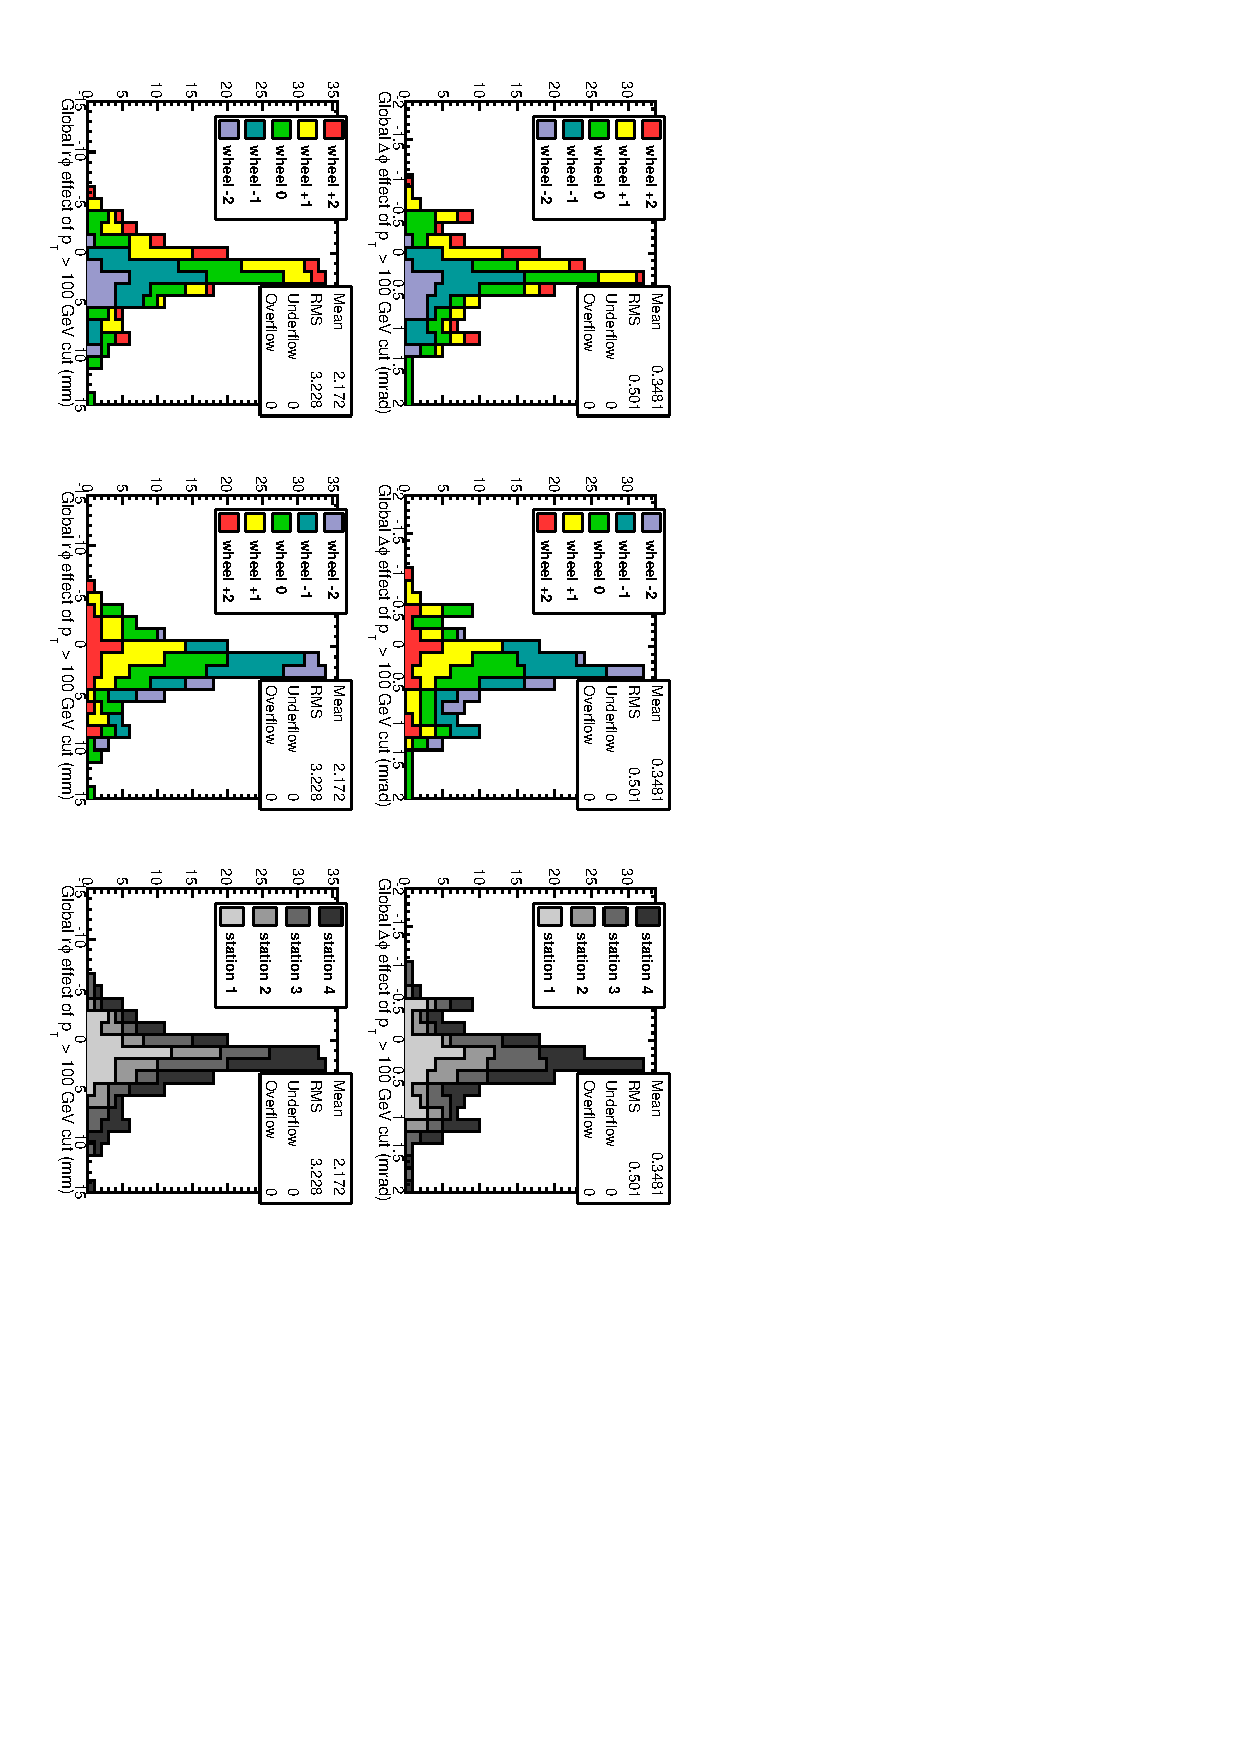
\includegraphics[height=\linewidth, angle=90]{data_effect_of_100GeVcut3.pdf}
\end{frame}

\begin{frame}
\frametitle{Studies of $p_T$ effect}
\framesubtitle{Alignments from low and high $p_T$ differ: how do we know which is right?}

\begin{itemize}
\item Ratio of tracker $p_T$ and globalMuon $p_T$ vs.\ momentum in CRAFT
\item Study repeated with low and high $p_T$ alignments {\scriptsize (from prev page)}
\item Alignment made with high $p_T$ (solid \textcolor{red}{red} and black) yields more correct ratios (1.0) at all momenta
\end{itemize}

\vfill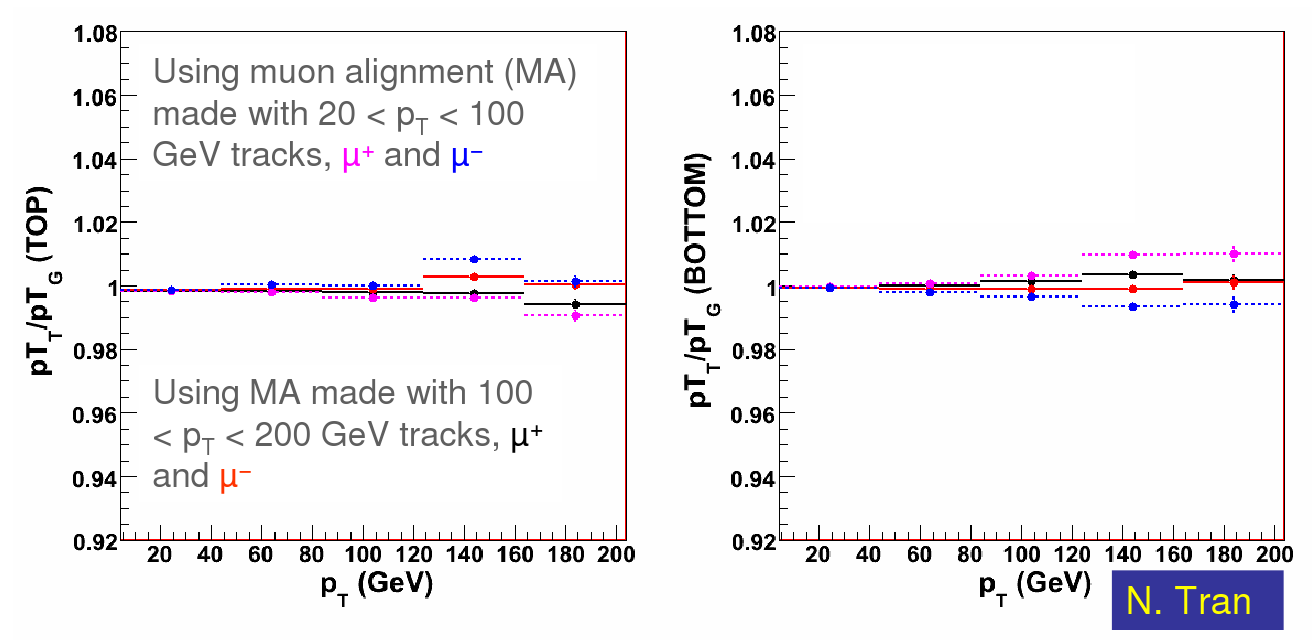
\includegraphics[width=\linewidth]{cosmicsplitting_nhan.png}
\end{frame}

\begin{frame}
\frametitle{Studies of $p_T$ effect}
\framesubtitle{Alignments from low and high $p_T$ differ: how do we know which is right?}
\scriptsize

\begin{itemize}
\item Cosmic track splitting: difference between top and bottom half of cosmic ray
\item Using high-$p_T$ alignment, tracks with station~1 muon hits (\textcolor{green}{TPFMS} and TMR) yield better resolution than \textcolor{red}{tracker only (TO)} for the first time!
\begin{itemize}\scriptsize
\item this was not the case for the low-$p_T$ alignment or any previous alignments
\end{itemize}
\item Highest-$p_T$ bin in this study \mbox{is statistically independent of 100--200~GeV alignment\hspace{-1 cm}}
\end{itemize}

\hfill \scriptsize \textcolor{darkblue}{J.~Tucker}

\vspace{-\baselineskip}
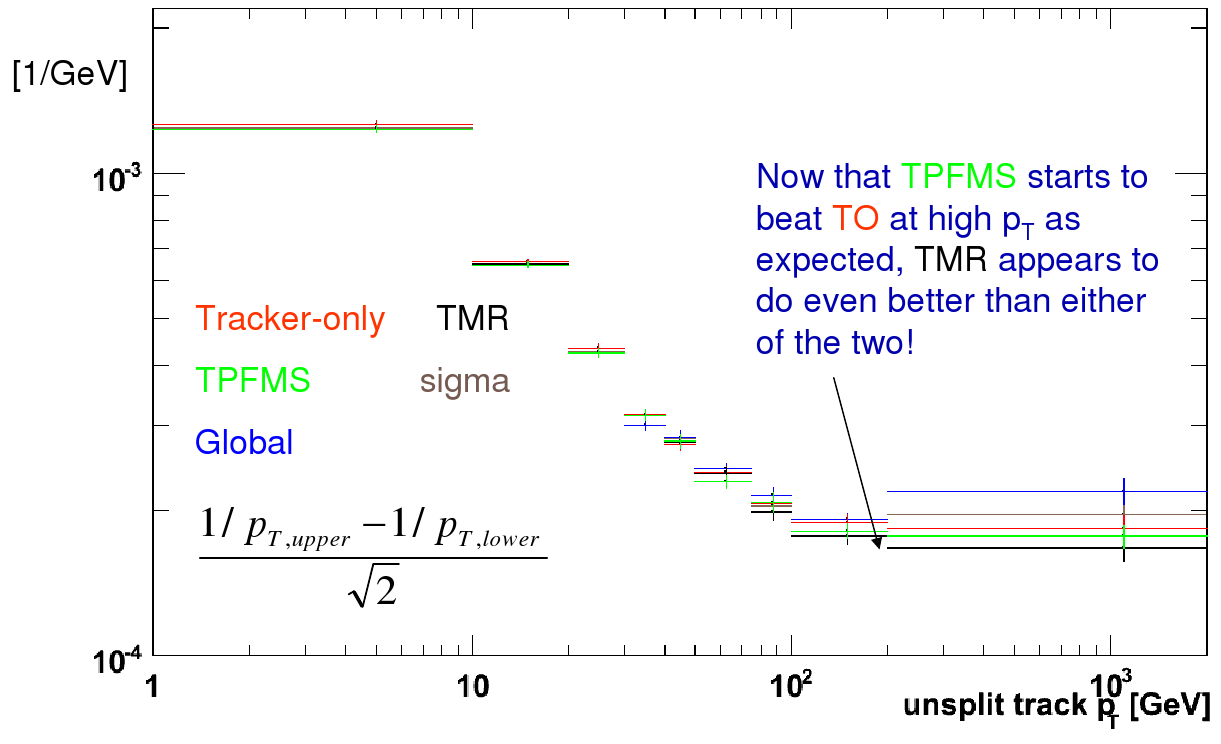
\includegraphics[width=0.87\linewidth]{cosmicsplitting_jordan.png}
\end{frame}

\begin{frame}
\frametitle{DB comparisons}

\begin{itemize}
\item CRAFT\_ALL\_V4 (before global alignment) minus new constants
\item Large spread is seen in absolute positions only; relative motion
  within sectors is much smaller
\end{itemize}

\vfill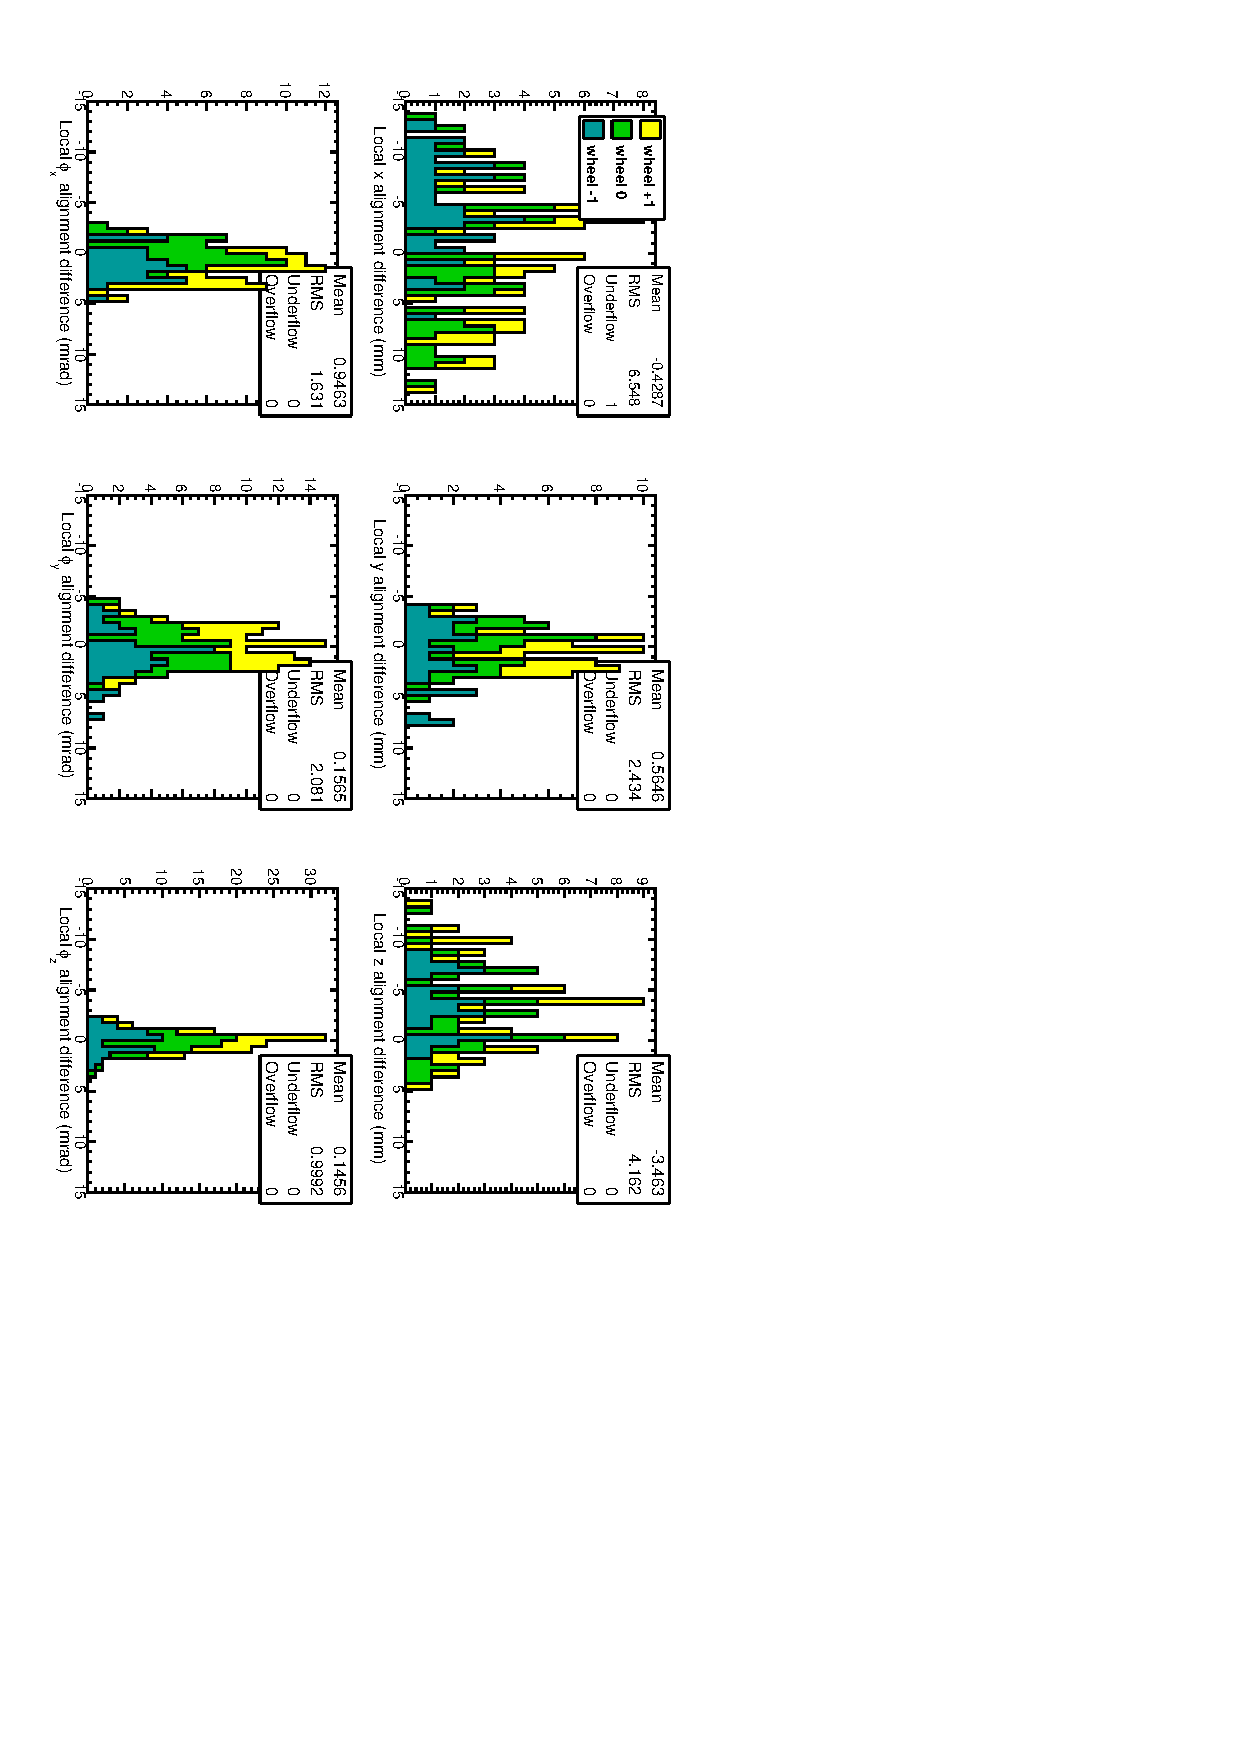
\includegraphics[height=\linewidth, angle=90]{hip_difference_v4.pdf}
\end{frame}

\begin{frame}
\frametitle{DB comparisons}

\begin{itemize}
\item CRAFT\_ALL\_V5--12 (first global alignment) minus new constants
\item Wheel-by-wheel dependence is the $p_T$ effect (new constants were produced with high-$p_T$)
\end{itemize}

\vfill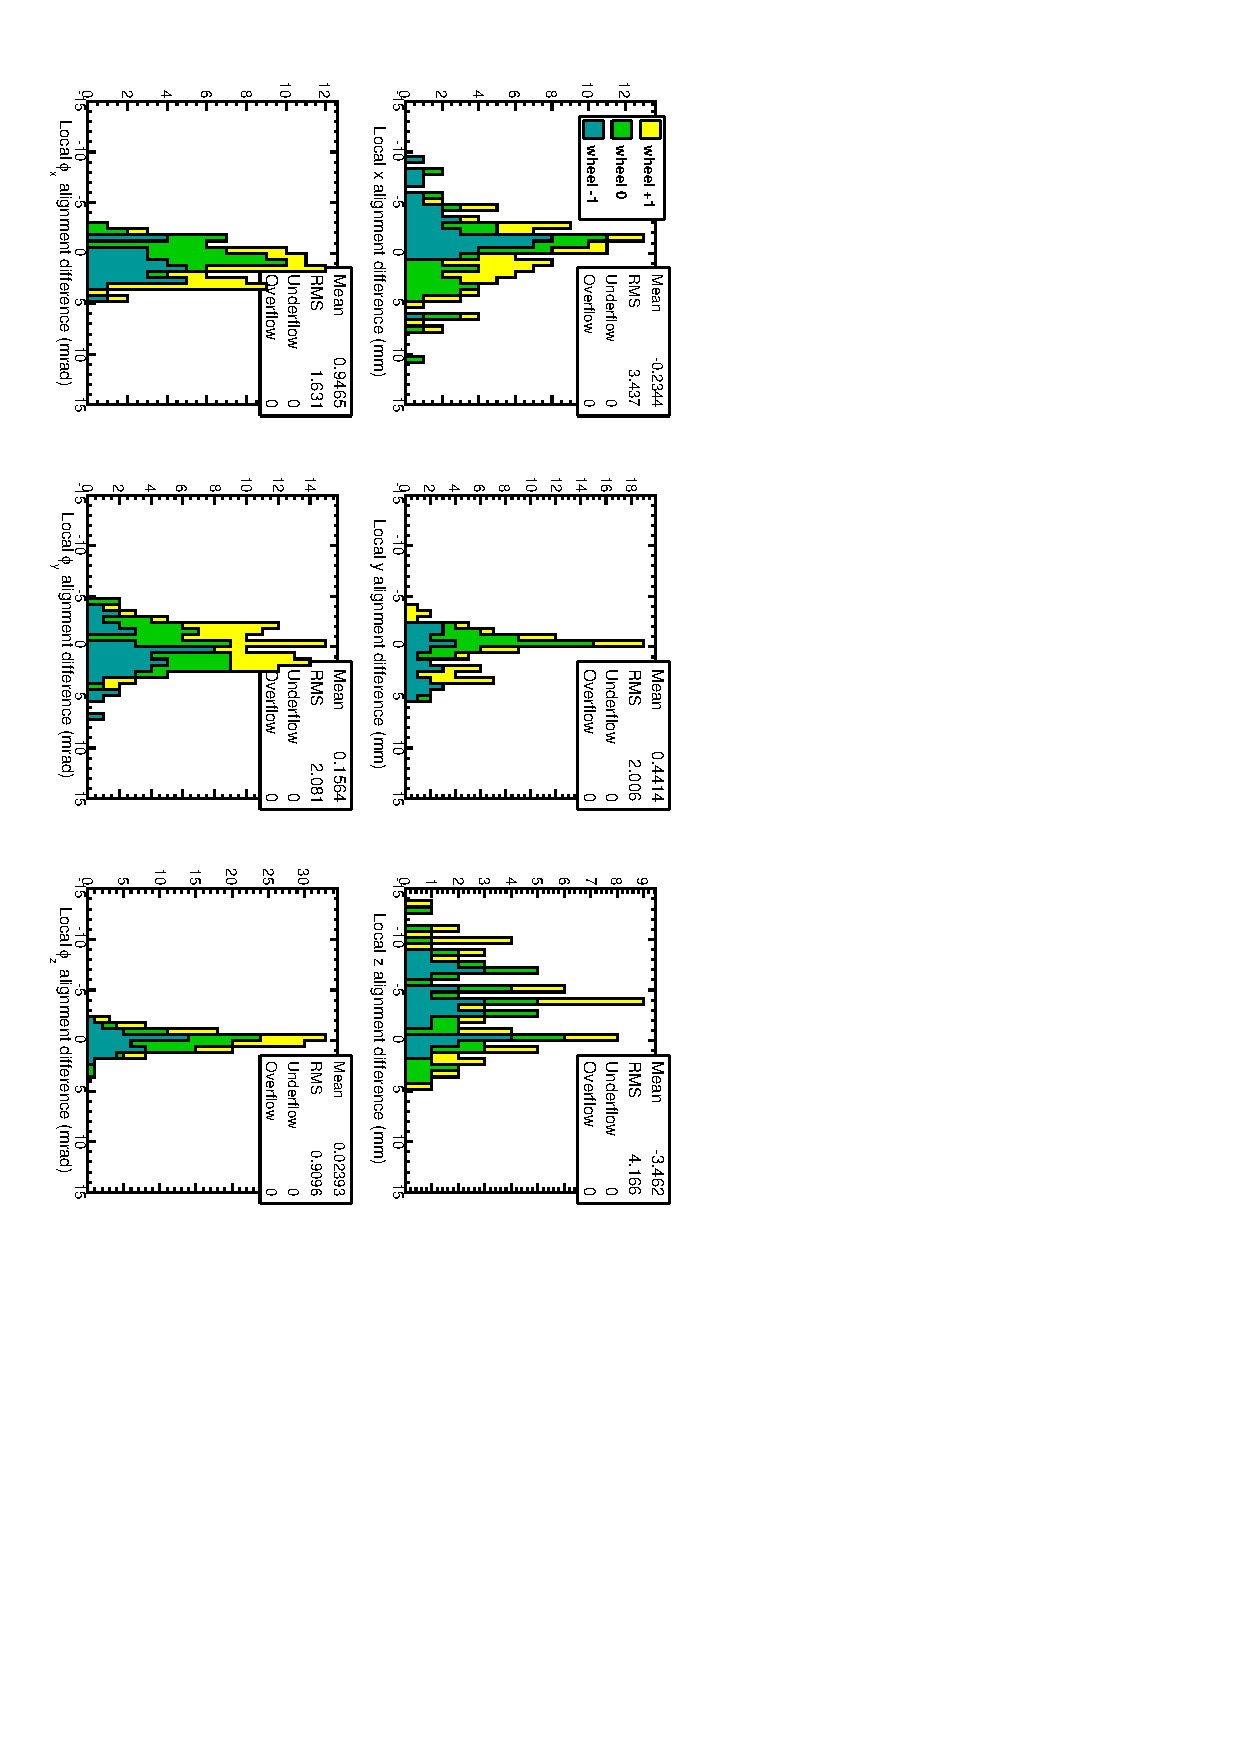
\includegraphics[height=\linewidth, angle=90]{hip_difference_v11all.pdf}
\end{frame}

\begin{frame}
\frametitle{Verification with segments}

\begin{itemize}
\item Test internal consistency of muon alignment by extrapolating segments from one station to the next
\item Relative local $x$ position mostly unchanged: sectors move together
\item $\sim$800~$\mu$m in stations 1--3
\item Outlier station~4 \textcolor{green}{(green)} chambers: possible internal misalignment
\end{itemize}

\vfill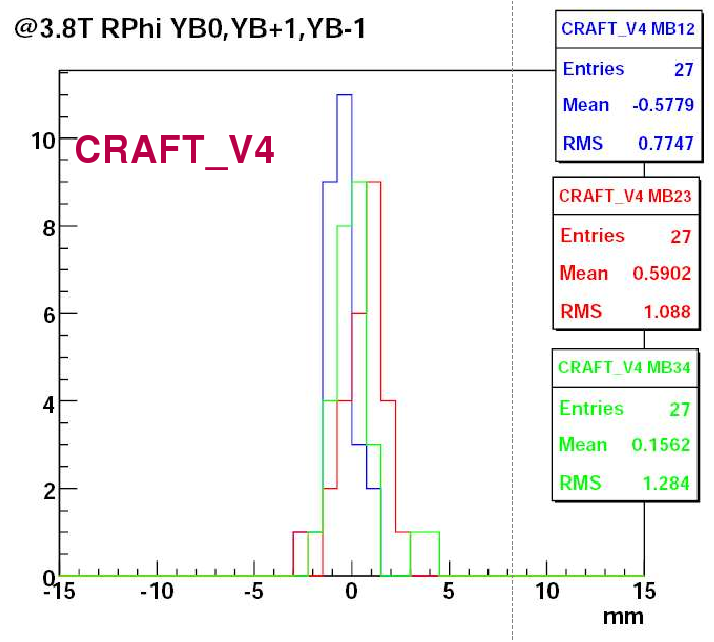
\includegraphics[width=0.5\linewidth]{alicia_v4_rphi.png}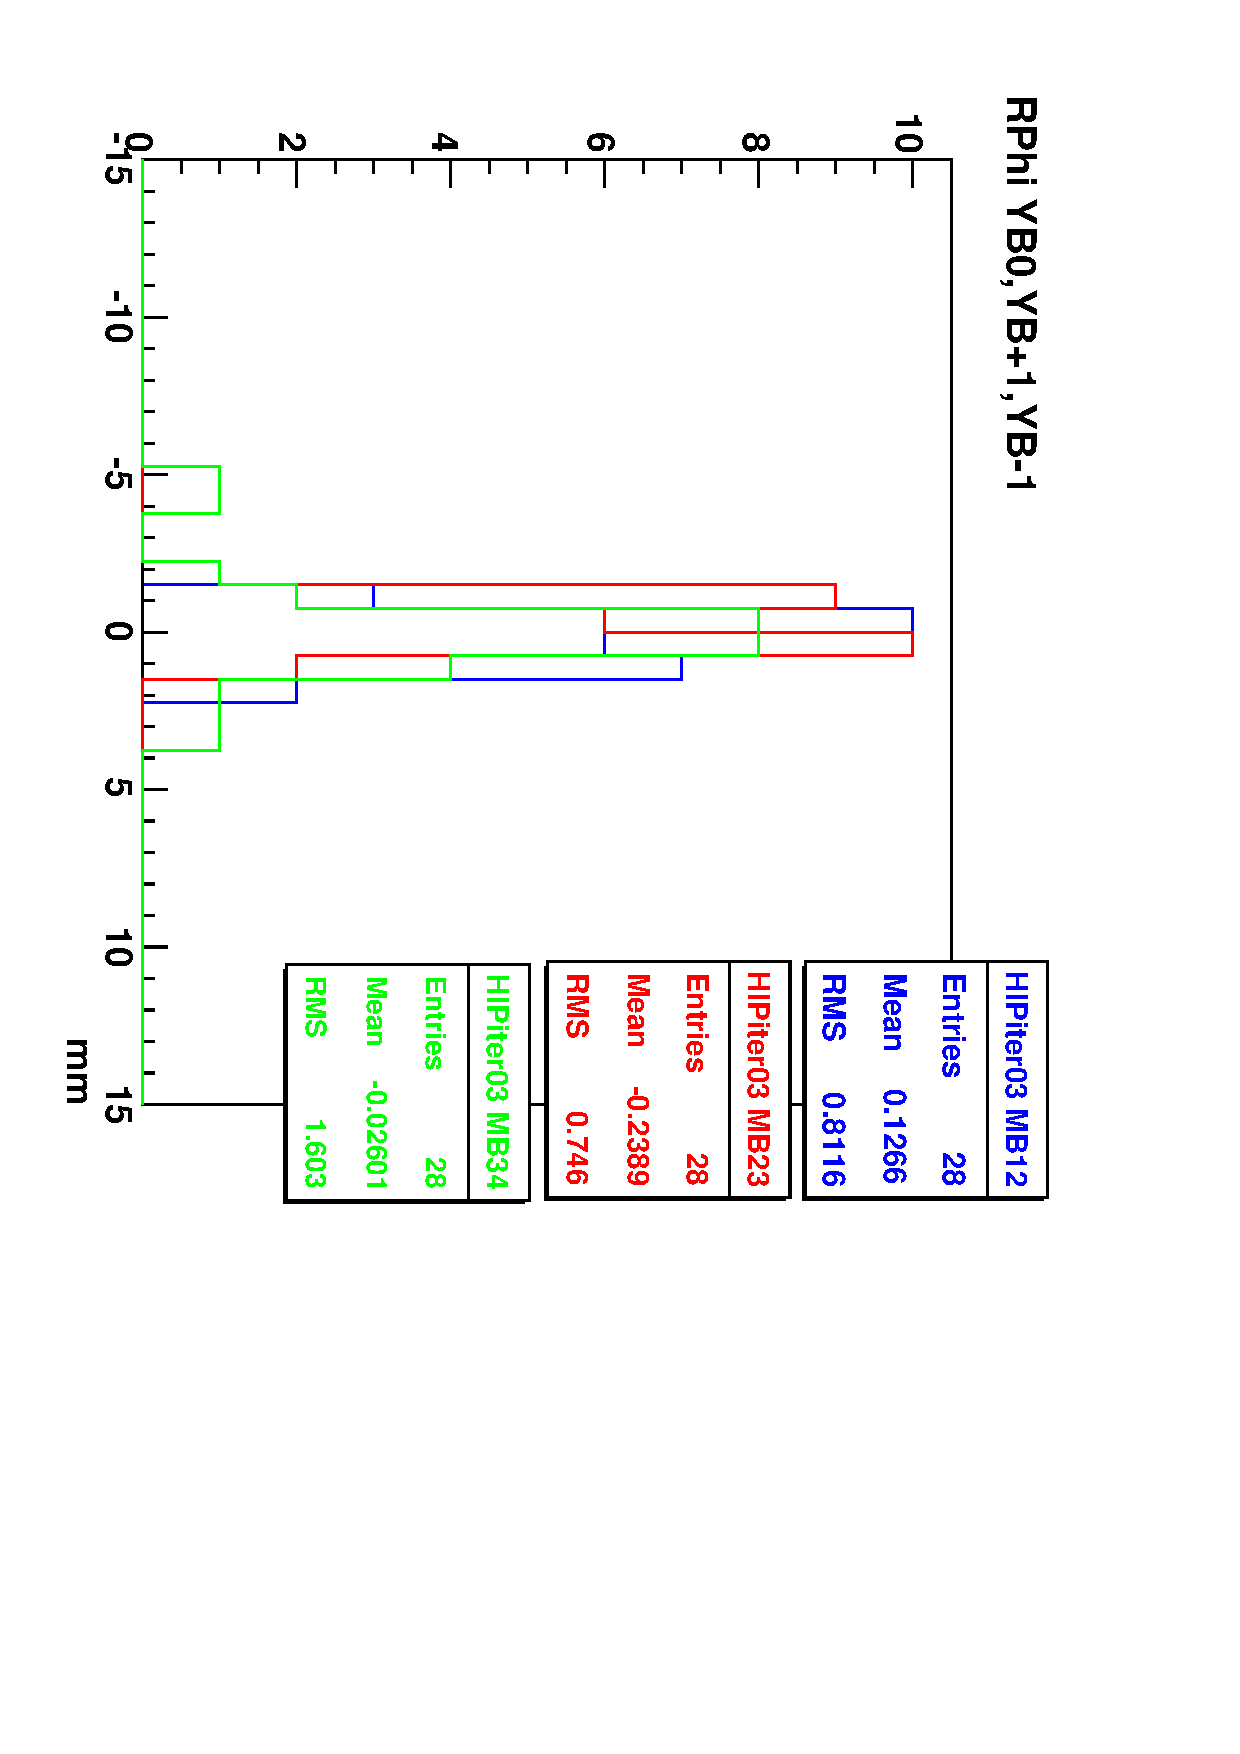
\includegraphics[height=0.5\linewidth, angle=90]{RPhires_YB0YB1YBm1_HIPiter03_InOut_38T-1.pdf}

\hfill \scriptsize \textcolor{darkblue}{A.~Calderon}
\end{frame}

\begin{frame}
\frametitle{Verification with segments}
\begin{itemize}
\item Relative local $\frac{dx}{dz}$ angle improved by almost a factor of 2
\item $\sim$0.7~mrad
\end{itemize}

\vfill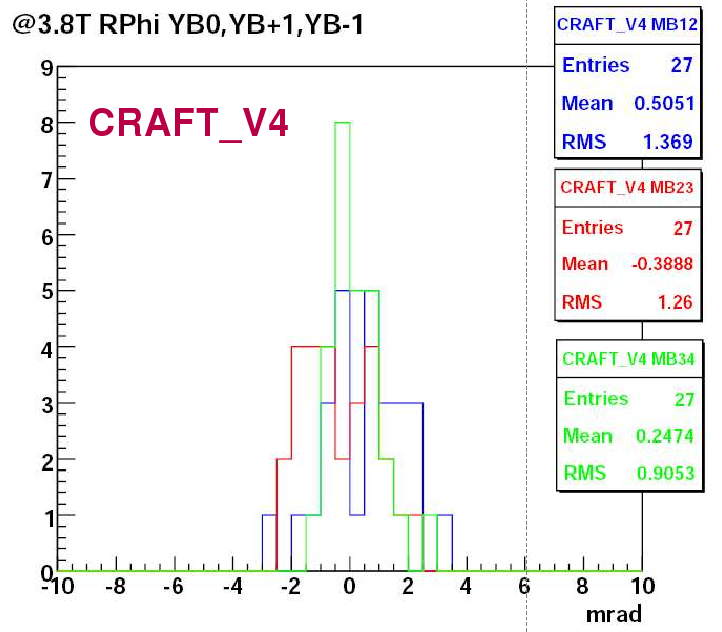
\includegraphics[width=0.5\linewidth]{alicia_v4_phiy.png}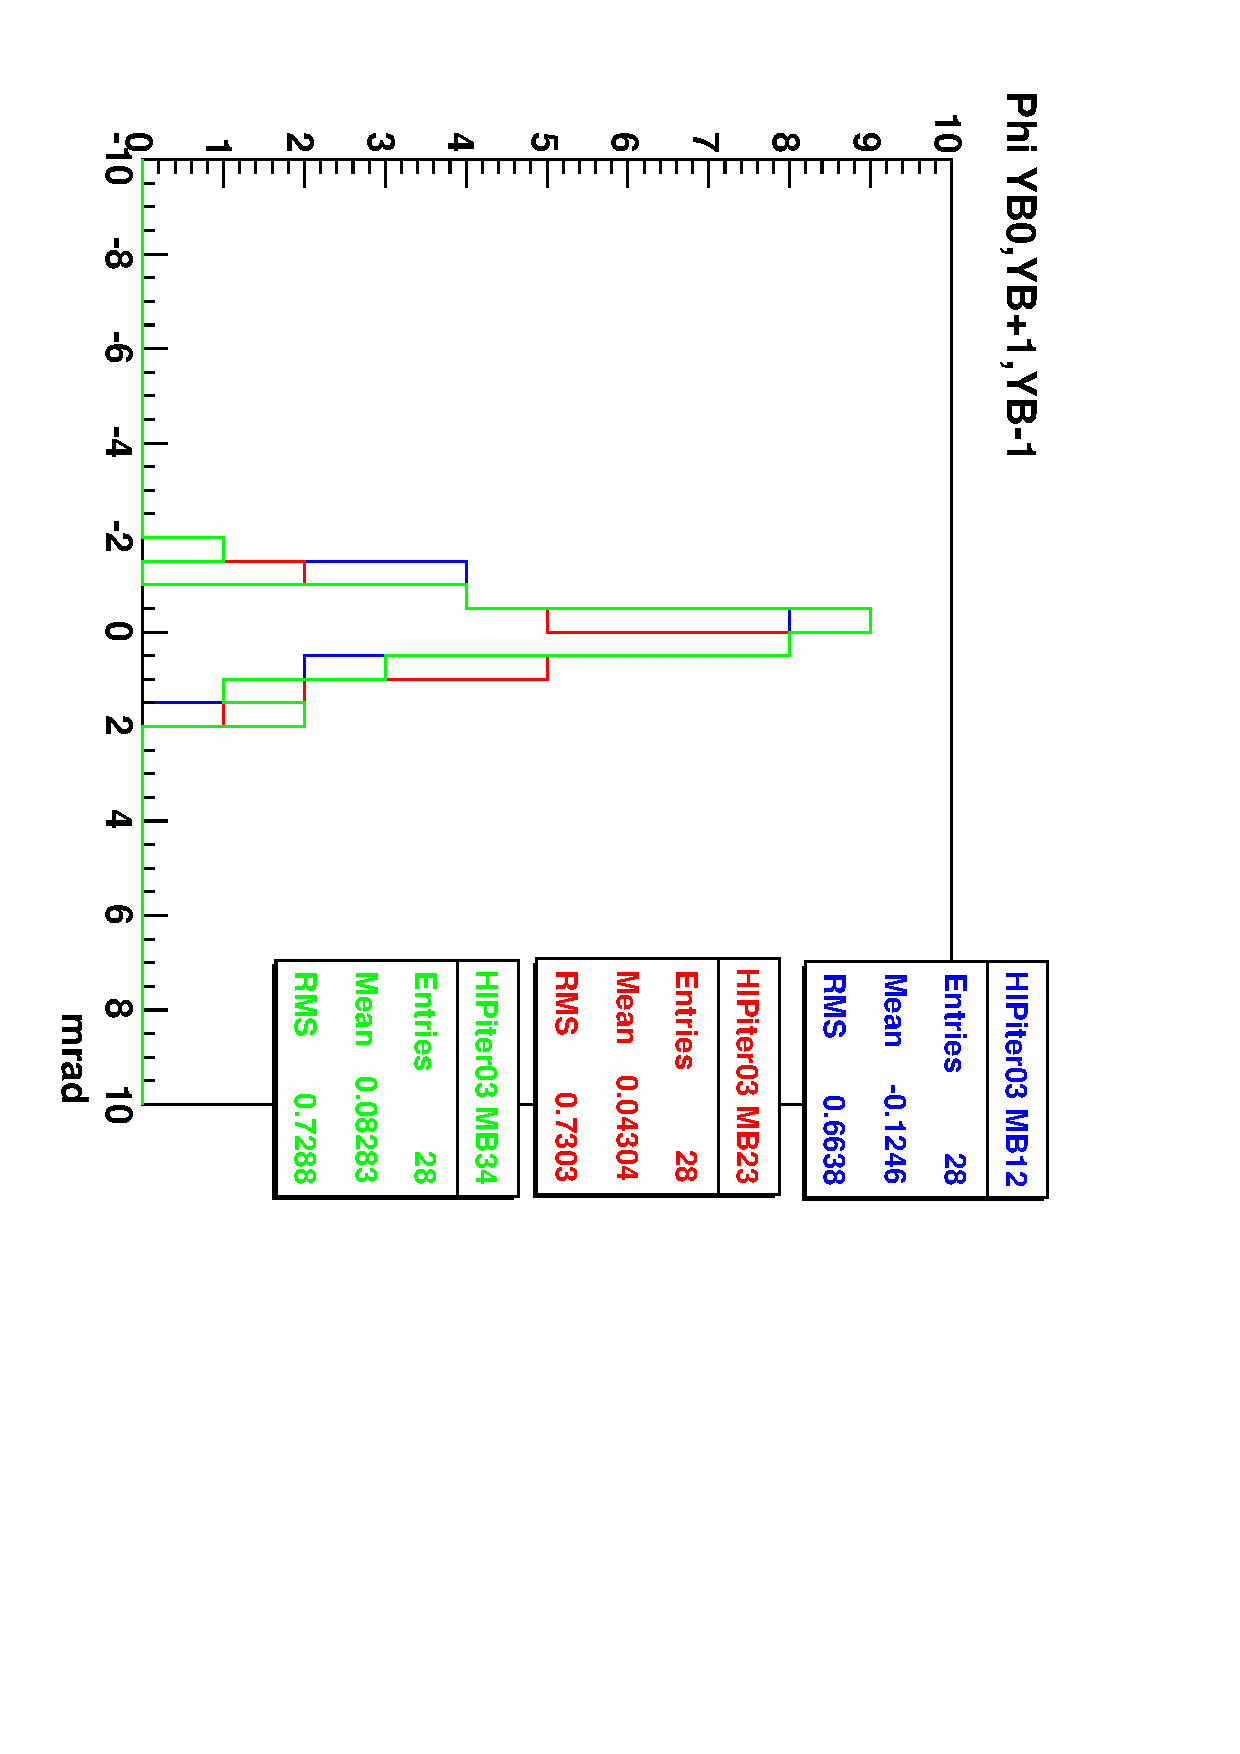
\includegraphics[height=0.5\linewidth, angle=90]{Phires_YB0YB1YBm1_HIPiter03_InOut_38T-1.pdf}

\hfill \scriptsize \textcolor{darkblue}{A.~Calderon}
\end{frame}

%% \section*{First section}
%% \begin{frame}
%% \begin{center}
%% \Huge \textcolor{blue}{First section}
%% \end{center}
%% \end{frame}

\begin{frame}
\frametitle{Conclusions}
\begin{itemize}\setlength{\itemsep}{0.3 cm}
\item New muon alignment constants are ready to be signed-off
\begin{itemize}\setlength{\itemsep}{0.15 cm}
\item internal DT alignment
\item hardware $+$ photogrammetry CSC alignment
\item global chamber alignment for DT wheels $-$1, 0, $+$1

{\scriptsize (pending final tracker alignment and APEs)}
\end{itemize}

\item New techniques allow for a more complete alignment: 6 DOF

\item Behavior studied in Monte Carlo: technique is sound and capable of 200~$\mu$m resolution

\item Real results verified by several independent techniques

\item Dependence of residuals on $p_T$ and $\frac{dx}{dz}$ (sawtooth) is still unexplained and exhibits global patterns ($p_T$-dependent rotation and twist)
\end{itemize}
\label{numpages}
\end{frame}

\begin{frame}
\frametitle{Tracker curl hypothesis}
\framesubtitle{$p_T$-dependent rotation could be curl in tracker, if large enough}
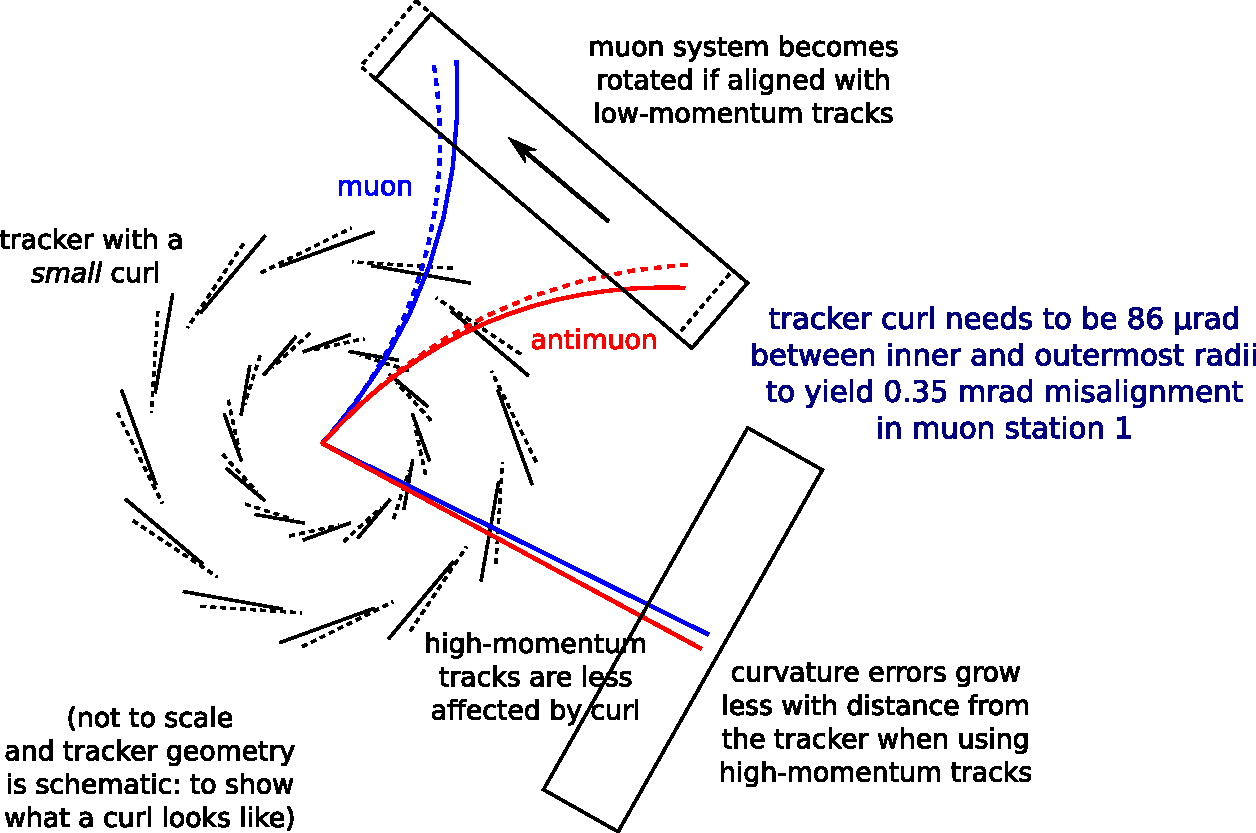
\includegraphics[width=\linewidth]{curl_explanation.pdf}
\end{frame}

\begin{frame}
\frametitle{Tracker curl constraints}

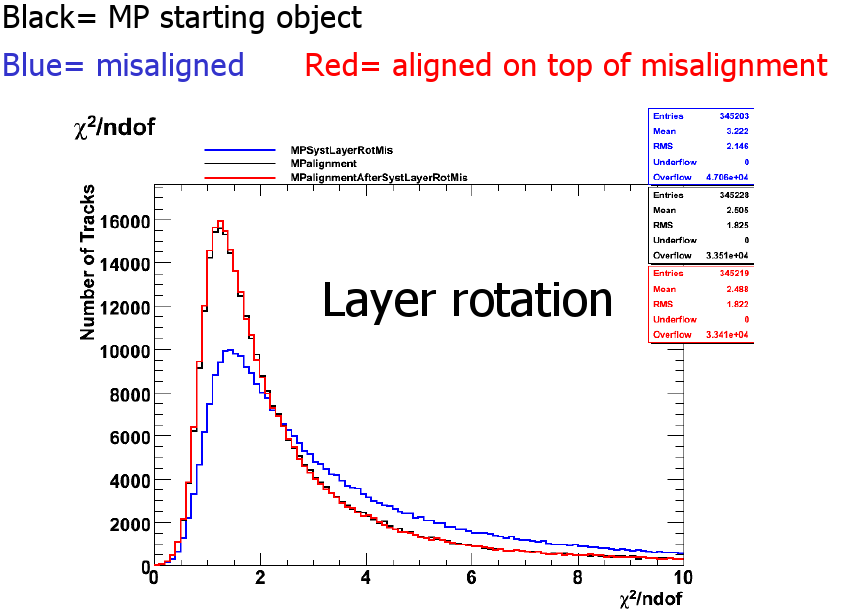
\includegraphics[width=0.55\linewidth]{tracks_are_sensitive_to_curl.png} \hfill 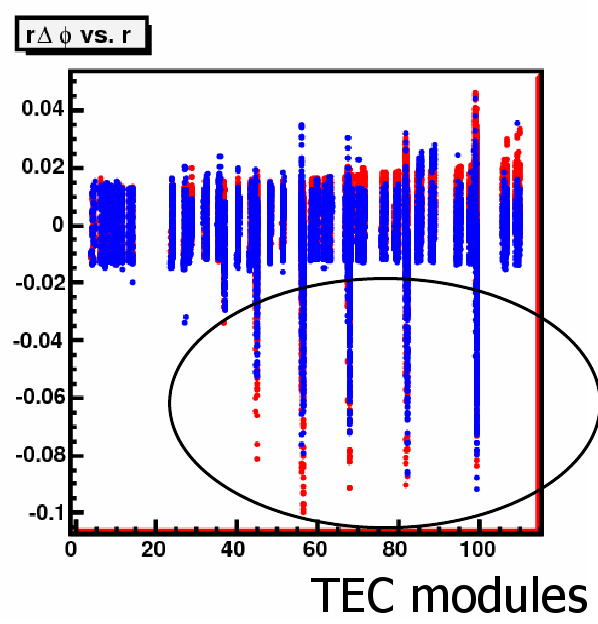
\includegraphics[width=0.35\linewidth]{curl_is_not_86microns.png}

\begin{itemize}
\item Studies performed in CRAFT data \hfill \textcolor{darkblue}{\scriptsize Zijin Guo, Roberto Castello}
\item \textcolor{darkblue}{Left:} tracker tracks are sensitive to 300~$\mu$rad curl (\textcolor{blue}{blue:\ adding curl worsens $\chi^2$} and \textcolor{red}{red:\ re-aligning restores it})
\item \textcolor{darkblue}{Right:} also restores wafer positions within 150~$\mu$rad \mbox{except TEC\hspace{-1 cm}}
\begin{itemize}
\item TEC not used in muon alignment; not relevant here
\item restored chamber positions randomly distributed around zero: \textcolor{darkblue}{no {\it systematic} trend on the scale of 86~$\mu$rad}
\end{itemize}
\end{itemize}
\end{frame}

\end{document}
